%SRS Document
%Copyright 2017 Yang LI
%https://github.com/zjzsliyang/42003201ObjectOrientedAnalysisAndDesign
%Under GPL-3.0 License

\documentclass[12pt]{scrreprt}
\usepackage{outline}
\usepackage{pmgraph}
\usepackage[normalem]{ulem}
\usepackage{graphicx}
\usepackage{verbatim}
\usepackage{hyperref}
\usepackage{color}
\usepackage{setspace}
\usepackage{tabularx}
\usepackage{float}
\title{

\includegraphics[width=0.8in]{DocumentRes/OnionExpress.png} \\
\vspace*{1in}
\textbf{Software Requirements Specification}}
\author{Yang LI\\
        Zhongjin LUO\\
        Guohui YANG\\
        Yirui WANG\\
        Xinying WU\\
        Yiqun LIN\\
		    \vspace*{0.5in} \\
		    School of Software Engineering\\
        \textbf{Tongji University}\\
        Group 4\\
}
\date{\today}

\setlength{\oddsidemargin}{0in}
\setlength{\evensidemargin}{0in}
\setlength{\topmargin}{0in}
\setlength{\headsep}{-.25in}
\setlength{\textwidth}{6.5in}
\setlength{\textheight}{8.5in}
\setlength{\parindent}{1cm}

\begin{document}
\maketitle
\tableofcontents

\chapter{Introduction}
Onion Express\textregistered\ is a system built for logistic companies,
which provides them with a solution to logistics tracking, goods packing,
goods distribution, after-sales management, data storage, information
processing, etc.

\section{Purpose}
These days as B2C business is increasing rapidly, the growth of
logistics business is also remarkable. The enormous market demand
brings logistics companies opportunities as well as the challenge.
Facing such kind of condition, this project is aimed at improving the
efficiency of field personnel and customer satisfaction of a logistics
company by building a cross-platform system.

\section{Definitions}
As Jobs has ever said, “People don't know what I really want at all,
until your products are in their eyes”. This project is specially
designed for an independent logistics companies like UPS. The business
scope is limited within China. To be more precise, the express is only
available in Jiangsu, Zhejiang and Shanghai at the beginning.
Temporarily private orders are not covered in the business scope,
which means the express company corporates with e-commercial companies only
with the cash-on-delivery express or normal express. The system focuses on logistics
service without regard to O2O, bulk cargo or self-support e-business.
Timing express might be expanded in future.

\section{System Overview}
The actors in the system are classified as \emph{Postman, E-business, Customer
service, Customer} and \emph{Agent}. \emph{Customer} and \emph{Agent} are
generalized as Receiver. The \emph{Postman} has access to this system
only on mobile devices while \emph{Customer} has access both on browsers
as well as mobile devices. \emph{E-business} offers orders periodically.
\emph{Customer service} helps to deal with tasks cannot be done only by
the system.\\
Web application and iOS application provide different functions for different
users to enhance user experience and have some humanization design(e.g.
using different colors to mark tasks as reception or delivery in postman’s app).
Besides basic functions, the system also provides some advanced functions,
like printing invoices. Different offline payment methods are supported.
And the customer’s telephone number is hidden to protect his/her privacy.\\
The postman is equipped with a multifunctional special device, when the
customer receives his/her package, he/she can use this device to pay by
card and can also press thumb on it to sign digitally, besides, the device
helps collect postman’s GPS location accurately.\\
The system considers all the 8 scenarios, including sending the package,
paying for the product, signing the package and so on. To integrate the
system, two scenarios are added. One is creating the orders, at the beginning
of the entire flow. Another is dealing the order manually, to reduce errors
caused by the system and handle other unanticipated situations. That can
improve the stability of the system and in consideration of the relatively
small scale of users in the early stage, robot customer service is not
necessary. It can be taken into consideration when the business is expanding
to a certain stage.\\
This project also designs several user interface mock-ups on the website
and on mobile devices. Core functions are exhibited in these mock-ups,
for example, the dispatch list interface.\\
Nonfunctional requirements and further explanations on security, performance,
data storage and computing, tracking the package, maintenance and others are
detailed in supplementary Specification.

\chapter{Use Case Modelling}
\section{Global Use Cases}
\begin{figure}[H]
  \centering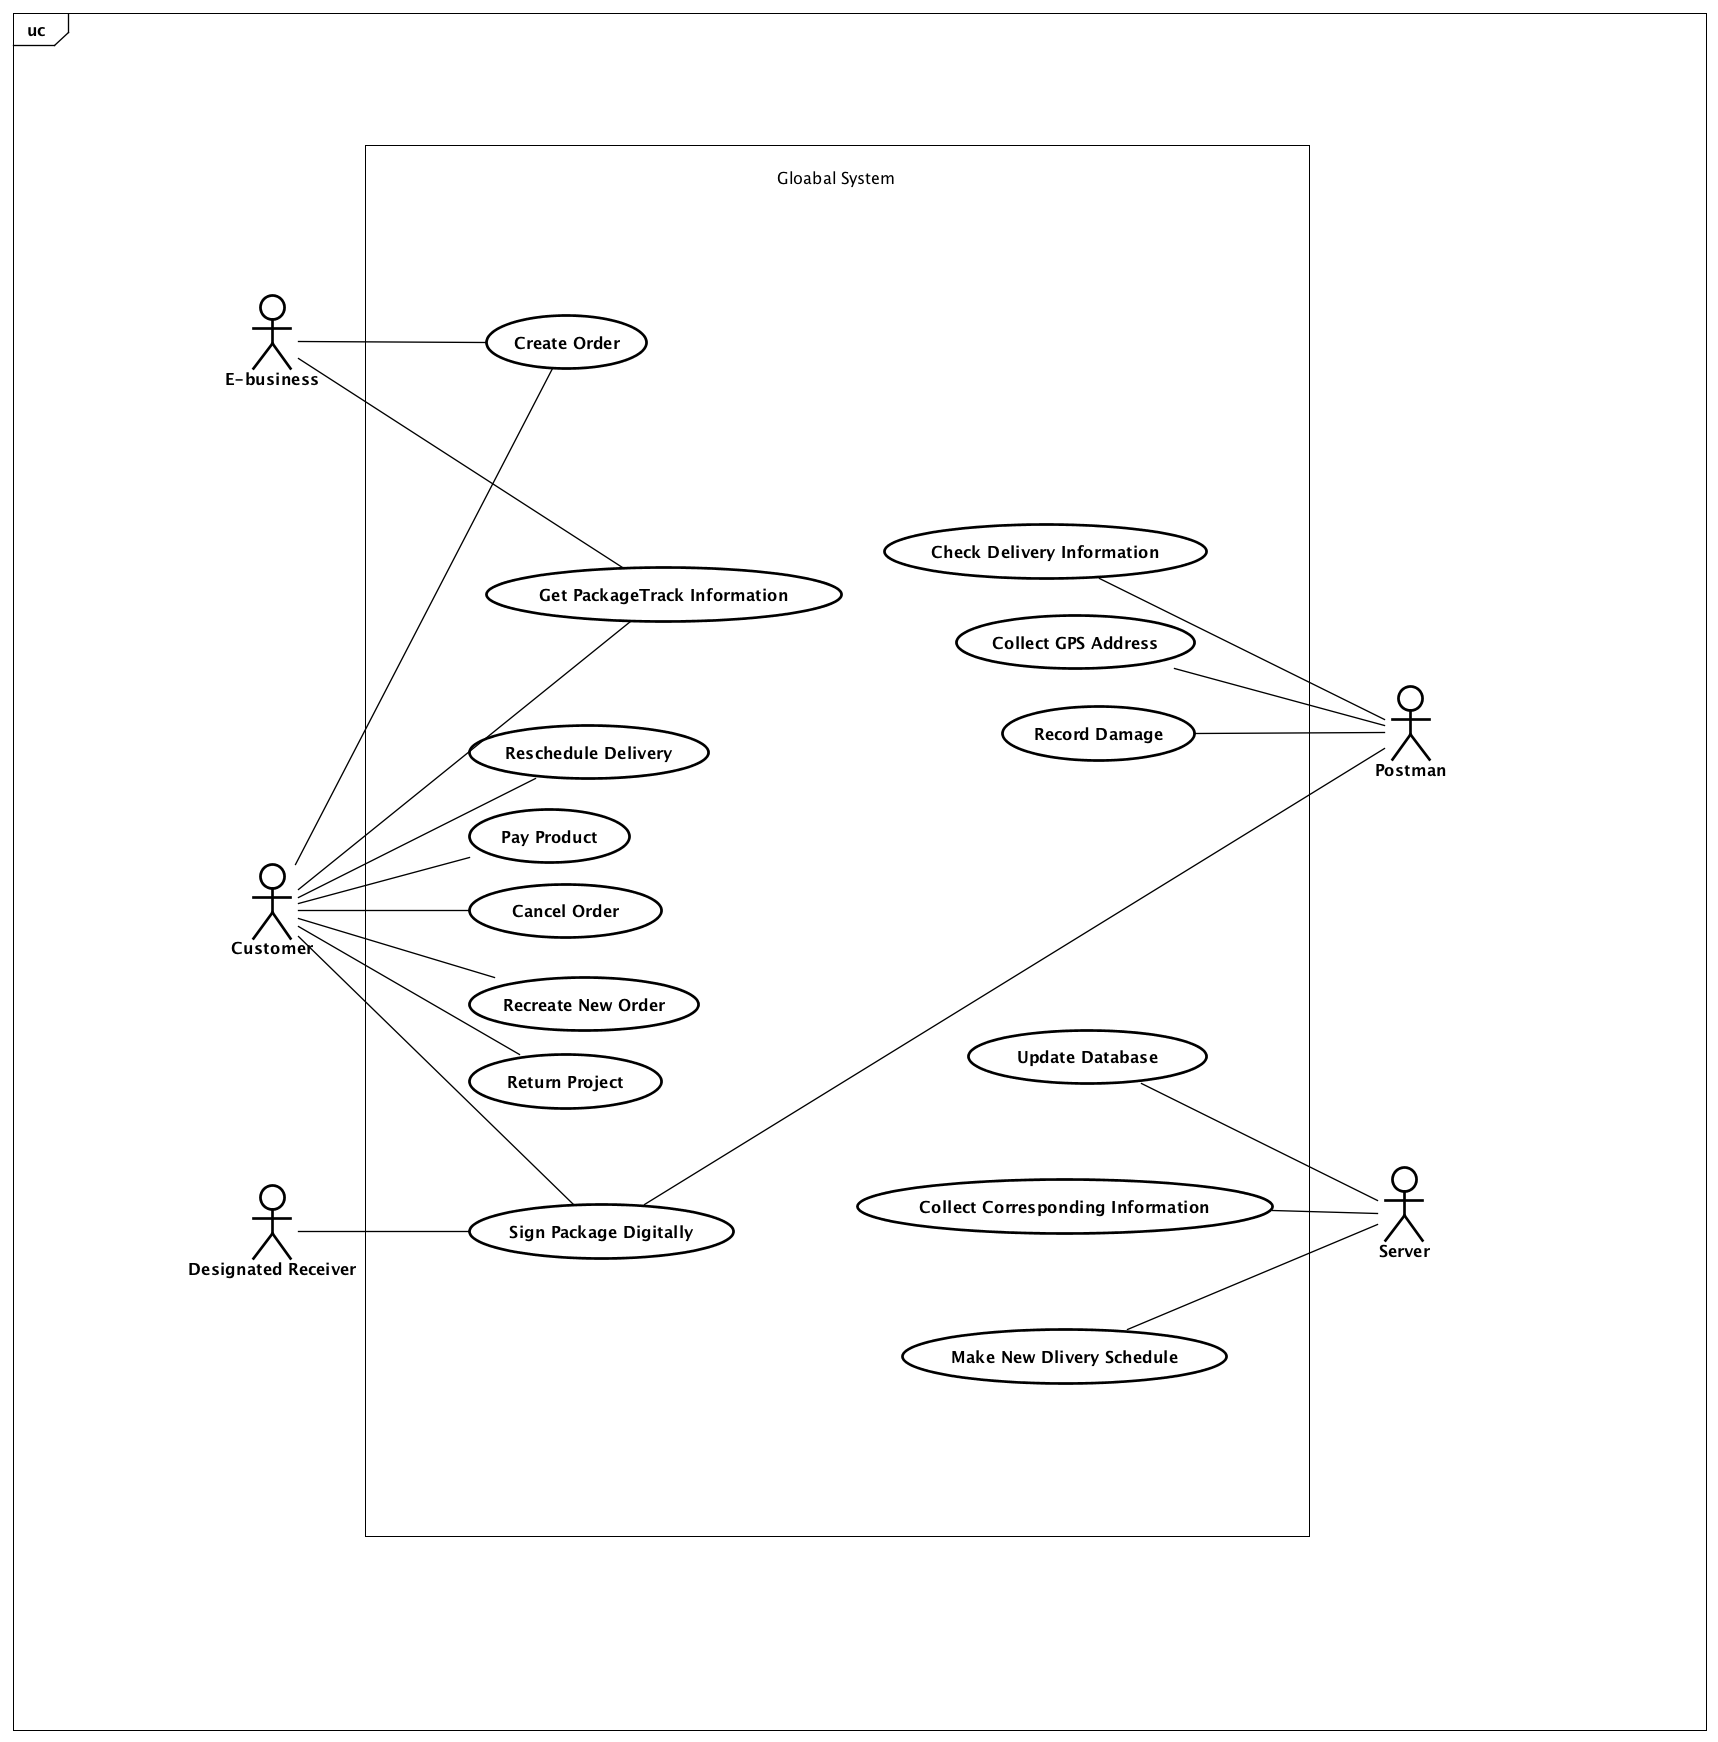
\includegraphics[width=5.5in]{DocumentRes/0UseCaseDiagram.png}
  \caption{Global Use Cases Diagram}
\end{figure}

\section{Specigication of Use Cases}
\subsection{Scenario One}
\begin{figure}[H]
  \centering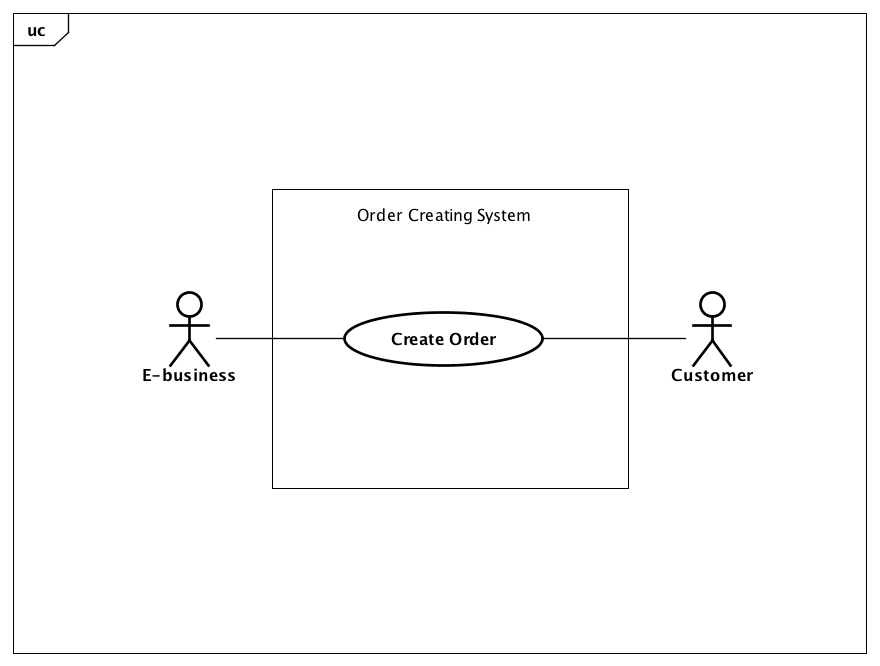
\includegraphics[width=4in]{DocumentRes/1UseCaseDiagram.png}
  \caption{Scenario One Use Case Diagram}
\end{figure}

\begin{table}
  \centering
  \begin{tabular}{| c | p{11cm} |}
    \hline
    Use Case Name & Create Order\\
    \hline
    Related Requirements & Scenario One\\
    \hline
    Goal in Context & The customer or E-business requests to create order.\\
    \hline
    Preconditions & The customer buys products from E-business or wants to
    send packages.\\
    \hline
    Successful End Condition & Server creates order according to the
    information provided by E-business \& Customer.\\
    \hline
    Failed End Condition & Server refuses to create an order.\\
    \hline
    Primary Actors & E-business and Customer\\
    \hline
    Secondary Actors & None\\
    \hline
    Trigger & E-business \& Customer sends the related information to Server.\\
    \hline
    Main Flow & Step 1 : Customer \& E-business Registers Information to Server.\\
    & Step 2 : Customer \& E-business Sends Information to Server.\\
    & Step 3 : Server checks whether the information is completed.\\
    & Step 4 : Server creates orders automatically according to the information above.\\
    & Step 5 : E-business \& customer transfers products to Logistics
    company and pays for the delivery. If the customer doesn’t pay before,
    Logistics company will pay for products for the customer in advance.\\
    & Step 6 : Logistics company transports packages to different regional
    distribution centers.\\
    \hline
    Extensions & The request of creating order is rejected.\\
    \hline
  \end{tabular}
\end{table}

\begin{figure}[H]
  \centering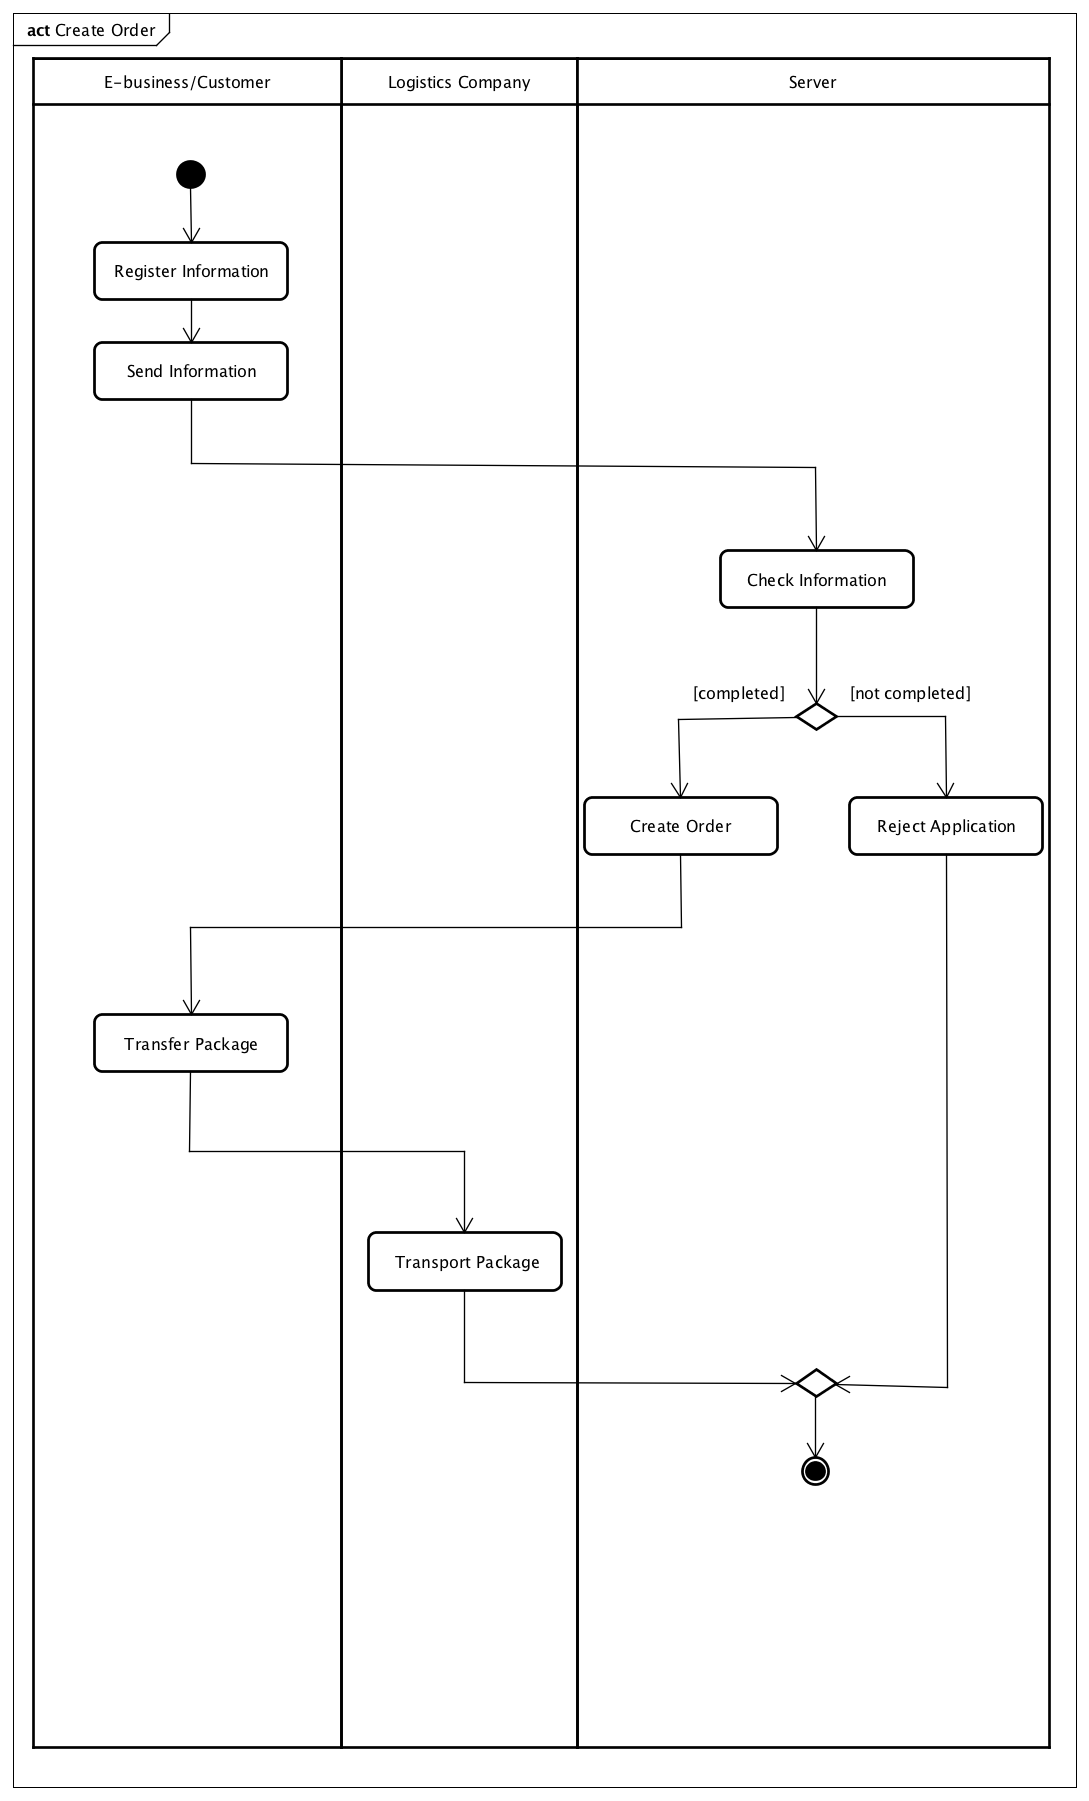
\includegraphics[width=5in]{DocumentRes/1ActivityDiagram.png}
  \caption{Scenario One Activity Diagram}
\end{figure}

\subsection{Scenario Two}
\begin{figure}[H]
  \centering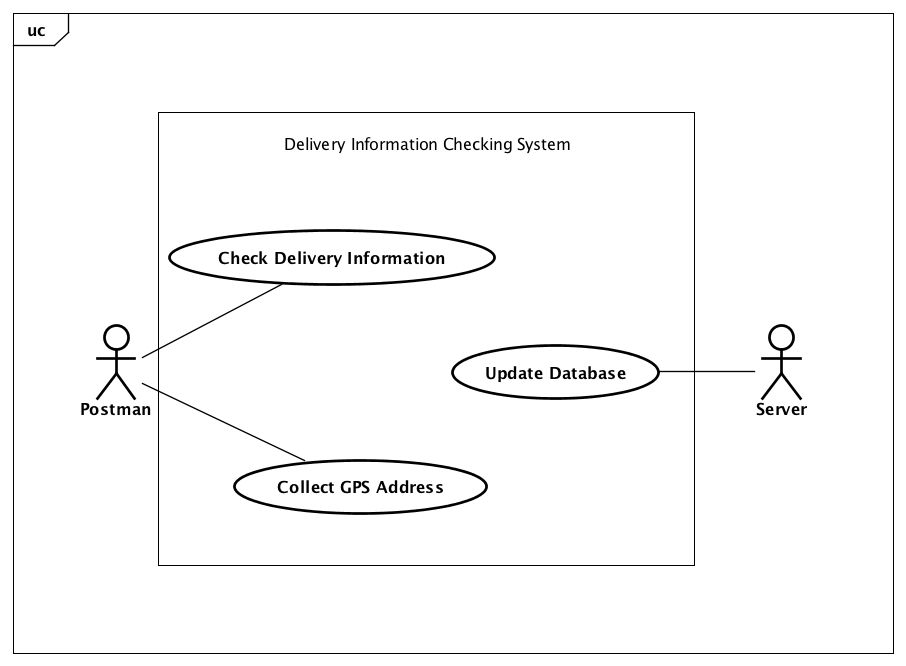
\includegraphics[width=4in]{DocumentRes/2UseCaseDiagram.png}
  \caption{Scenario Two Use Case Diagram}
\end{figure}

\begin{table}[H]
  \centering
  \begin{tabular}{| c | p{11cm} |}
    \hline
    Use Case Name & Collect GPS Address\\
    \hline
    Related Requirements & Scenario One\\
    \hline
    Goal in Context & Postmen collect the GPS address of the customer.\\
    \hline
    Preconditions & Postmen have delivered packages to the destination.\\
    \hline
    Successful End Condition & Server Updates database successfully.\\
    \hline
    Failed End Condition & None\\
    \hline
    Primary Actors & Postman\\
    \hline
    Secondary Actors & Server\\
    \hline
    Trigger & The GPS address of  the customer is not in the database.\\
    \hline
    Main Flow & Step 1 : Postmen inspect that whether the GPS address of
    the customer is in the database.\\
    & Step 2 : If the GPS address of  the customer is not in the database,
    postmen will collect the GPS address.\\
    & Include : Update database.\\
    \hline
    Extensions & None\\
    \hline
  \end{tabular}
\end{table}

\begin{table}
  \centering
  \begin{tabular}{| c | p{11cm} |}
    \hline
    Use Case Name & Check Delivery Information\\
    \hline
    Related Requirements & Scenario Two\\
    \hline
    Goal in Context & Postmen accept delivery task assigned by the system.\\
    \hline
    Preconditions & Orders have been created and packages have been
    transported to the regional distribution centers.\\
    \hline
    Successful End Condition & Postmen check delivery information and send
    packages to the customer.\\
    \hline
    Failed End Condition & None\\
    \hline
    Primary Actors & Postman\\
    \hline
    Secondary Actors & None\\
    \hline
    Trigger & Postmen accept an delivery task.\\
    \hline
    Main Flow & Step 1 : Logistics Company assigns task to Postman.\\
    & Step 2 : Postmen accept delivery task.\\
    & Step 3 : Postmen log in the system.\\
    & Step 4 : Postmen check delivery information including tracking number,
    destination, personal information about receivers, QR code for payment
    (if the customer choose to pay on-site) and so on.\\
    & Step 5 : Postmen go to the regional distribution center and get the
    package.\\
    & Step 6 : Postmen deliver it to the destination.\\
    & Step 7 : Postmen inform customers to take packages. At the same time,
    Postmen will Inspect Address, if the GPS address of  the customer is not
    in the database, they will collect the GPS address.\\
    \hline
    Extensions & None\\
    \hline
  \end{tabular}
\end{table}

\begin{table}
  \centering
  \begin{tabular}{| c | p{11cm} |}
    \hline
    Use Case Name & Update Database\\
    \hline
    Goal in Context & Server Updates database.\\
    \hline
    Preconditions & Postmen collected the GPS address of  the customer and
    sended to server.\\
    \hline
    Successful End Condition & Server Updates database successfully.\\
    \hline
    Failed End Condition & Server fails to update database.\\
    \hline
    Primary Actors & Server\\
    \hline
    Secondary Actors & None\\
    \hline
    Trigger & The GPS address of  the customer is not in the database.\\
    \hline
    Main Flow & Step 1 : Server Updates database.\\
    \hline
    Extensions & None\\
    \hline
  \end{tabular}
\end{table}

\begin{figure}[H]
  \centering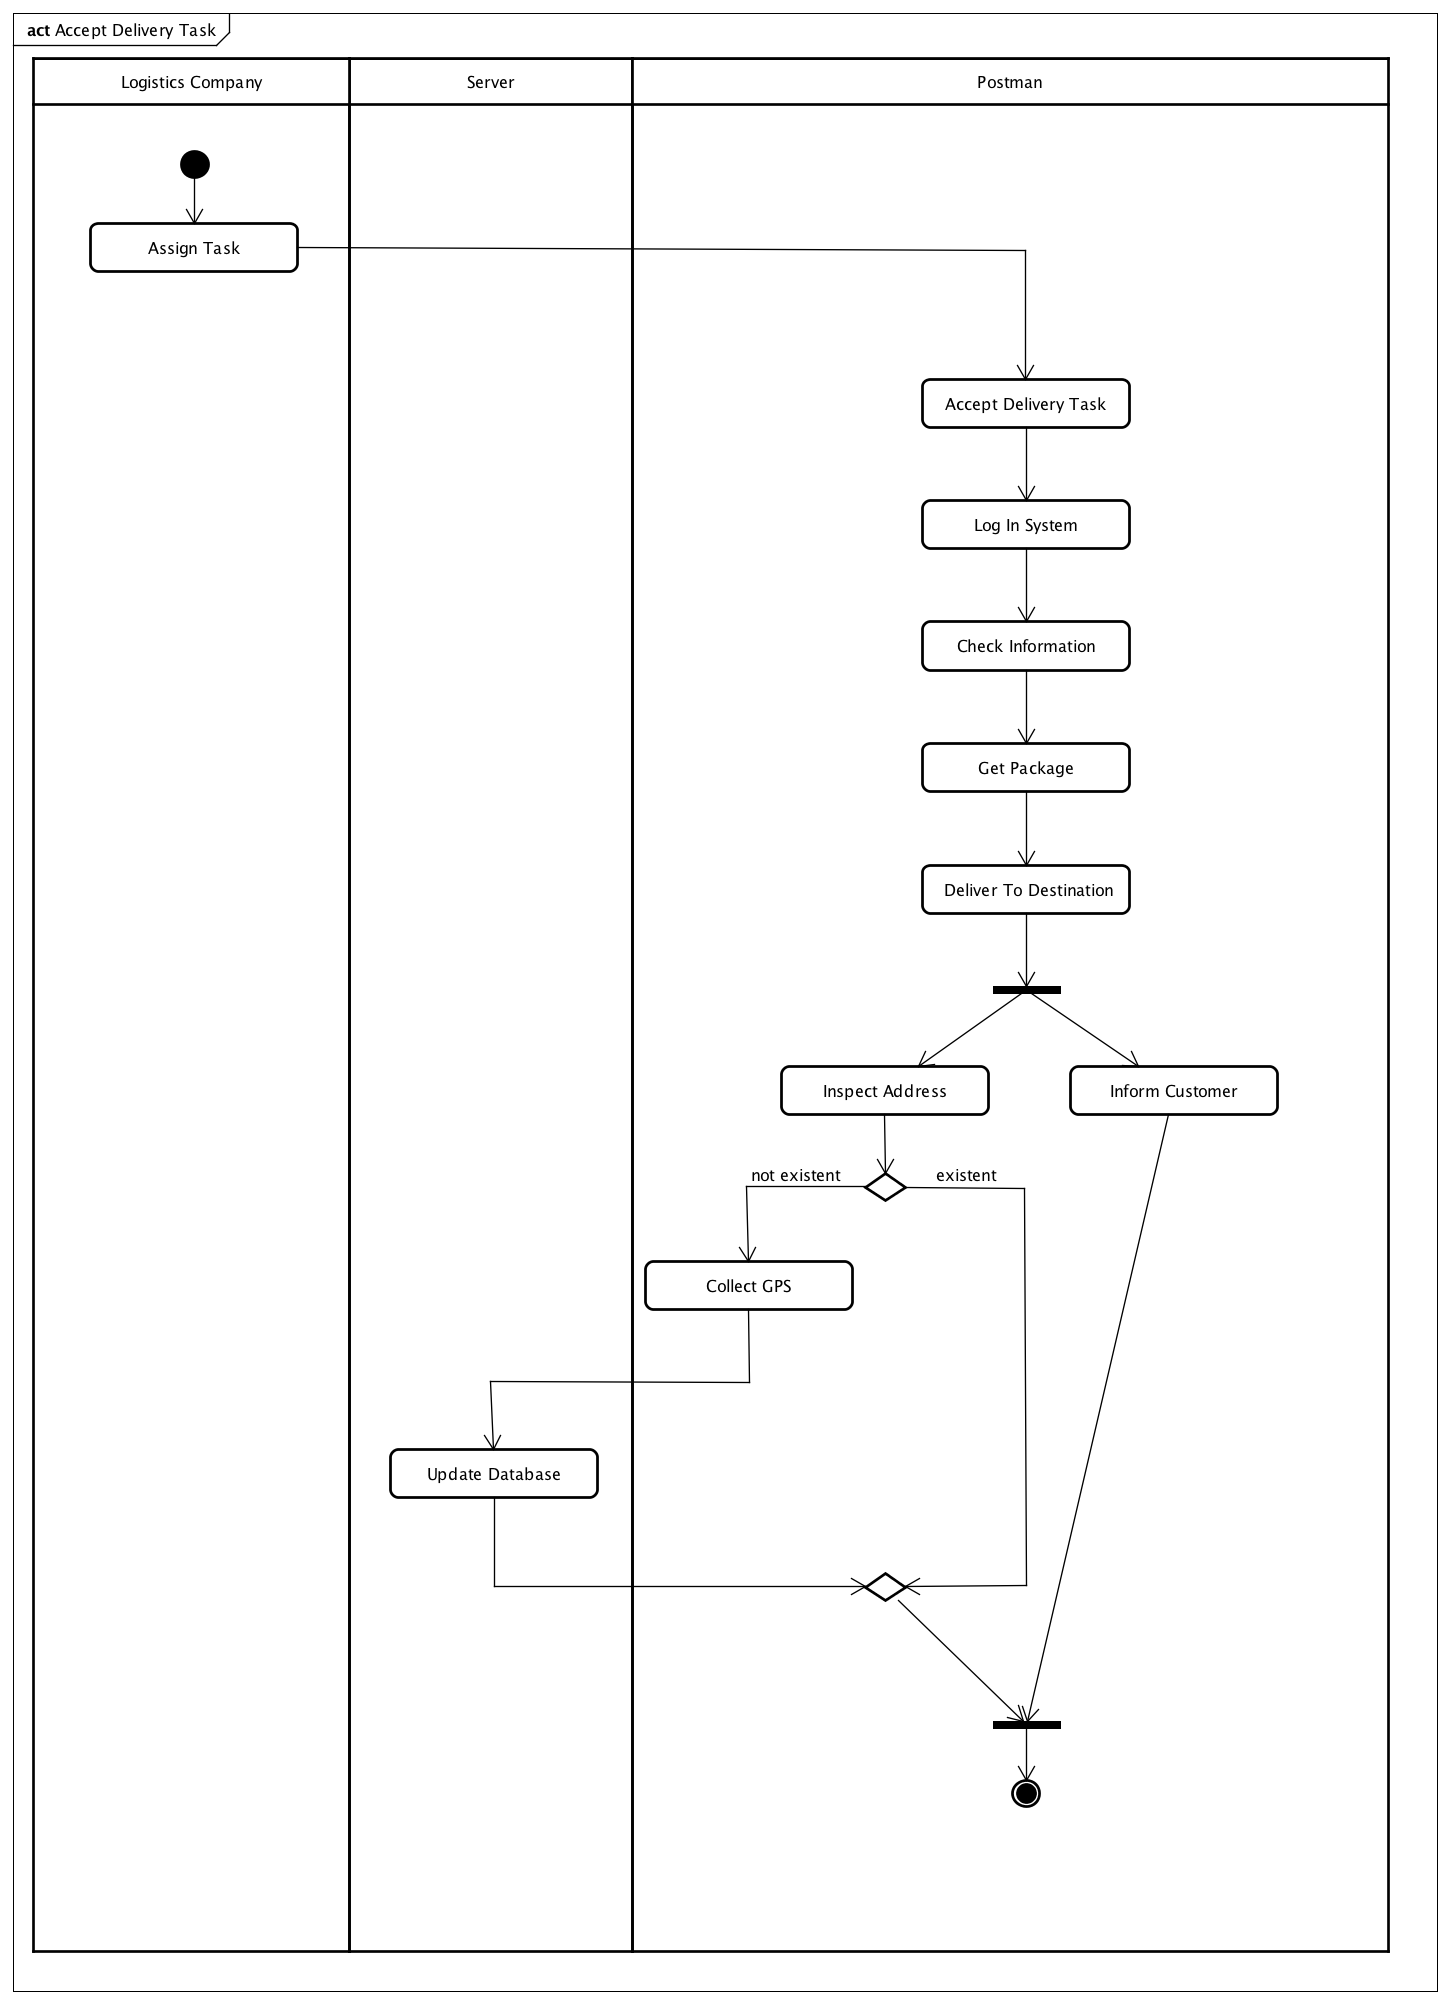
\includegraphics[width=5in]{DocumentRes/2ActivityDiagram.png}
  \caption{Scenario Two Activity Diagram}
\end{figure}

\subsection{Scenario Three}
\begin{figure}[H]
  \centering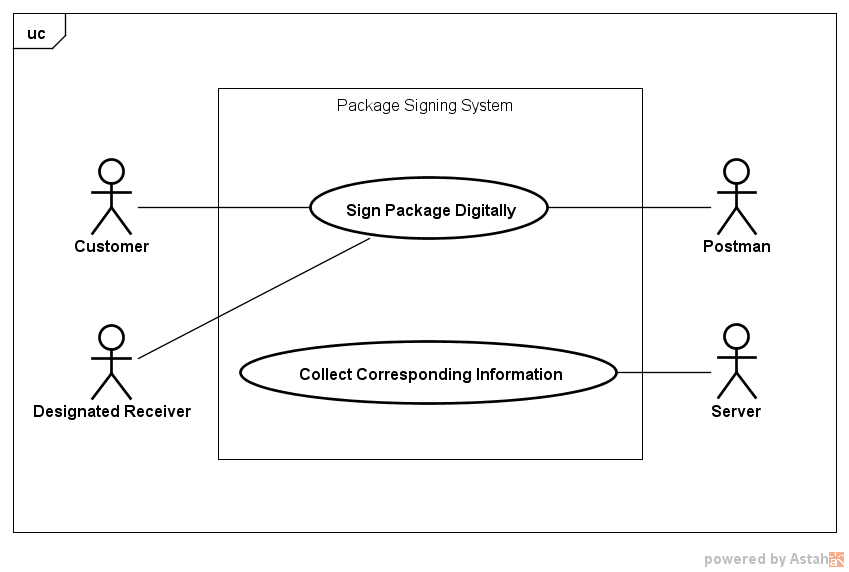
\includegraphics[width=4in]{DocumentRes/3UseCaseDiagram.png}
  \caption{Scenario Three Use Case Diagram}
\end{figure}

\begin{table}[H]
  \centering
  \begin{tabular}{| c | p{11cm} |}
    \hline
    Use Case Name & Collect Corresponding Information\\
    \hline
    Related Requirements & Scenario Two \& Three\\
    \hline
    Goal in Context & Collect information and archive related data.\\
    \hline
    Preconditions & Signing package is finished successfully.\\
    \hline
    Successful End Condition & The order is marked as complete; Relavant
    information is gathered.\\
    \hline
    Failed End Condition & The order is unfinished; Inspect system exception.\\
    \hline
    Primary Actors & Server\\
    \hline
    Secondary Actors & None\\
    \hline
    Trigger & System sends server a message that informs the package delivery
    is done.\\
    \hline
    Main Flow & Step 1 : Information including the data of received products,
    customer acceptance and some other transaction details are collected by
    the server. All necessary related data is archived to database.\\
    & Step 2 : Server requests to mark this order as complete.\\
    \hline
    Extensions & Step 1.1 : Error appears upon the procedure of data
    collection.\\
    & Step 1.2 : Data collection is undone.\\
    \hline
  \end{tabular}
\end{table}

\begin{table}
  \centering
  \begin{tabular}{| c | p{11cm} |}
    \hline
    Use Case Name & Confirm Reception\\
    \hline
    Related Requirements & Scenario Two \& Three\\
    \hline
    Goal in Context & Customer verifies if the receiver is designated
    by him/her.\\
    \hline
    Preconditions & The package has delivered to the customer-specified
    location on time but customer is not convenient to received it.\\
    \hline
    Successful End Condition & The receiver has the permission to sign the
    package.\\
    \hline
    Failed End Condition & The receiver is an imposter; Postman refuses giving
    him/her the package.\\
    \hline
    Primary Actors & Customer\\
    \hline
    Secondary Actors & Postman\\
    \hline
    Trigger & Someone but not customer claims that he/she have the permission
    to receive the package.\\
    \hline
    Main Flow & Step 1 : Postman collects the necessary information of that
    person and then sends to customer.\\
    & Step 2 : Customer confirms the if the potential receiver is as expected.\\
    & Step 3 : Postman gets a positive feedback from customer.\\
    & Step 4 : The receiver can sign the package under customer's permission.\\
    \hline
    Extensions & Step 3.1 : Postman gets a negative feedback from customer;
    That person is an imposter.\\
    & Step 3.2 : Postman refuses to give away the parcel.\\
    \hline
  \end{tabular}
\end{table}

\begin{table}
  \centering
  \begin{tabular}{| c | p{11cm} |}
    \hline
    Use Case Name & Sign on Pad\\
    \hline
    Related Requirements & Scenario Two \& Three\\
    \hline
    Goal in Context & A customer or the receiver designated by him/her requests
    to sign his/her name (or other proofs of identity) on Pad.\\
    \hline
    Preconditions & The package has delivered to the customer-specified
    location on time.\\
    \hline
    Successful End Condition & The customer receives the package; Package
    delivery success.\\
    \hline
    Failed End Condition & The customer fails to get the package; Package
    should be returned or reschedule delivery.\\
    \hline
    Primary Actors & Customer, Package receiving representative.\\
    \hline
    Secondary Actors & Postman\\
    \hline
    Trigger & Postman requests customer to sign on pad with the agreetment of
    customer.\\
    \hline
    Included Cases & Confirm Reception, Collect Corresponding Information\\
    \hline
    Main Flow & Step 1 : Customer checks if the parcel is delivered right
    and in good condition in person.\\
    & Step 2 : Customer signs on pad.\\
    & Step 3 : Postman confirms the package is received by customer or his/her
    representative.\\
    & Step 4 : All corresponding information including the data of the received
    product and customer acceptance will be transferred back to the server;
    The order will be marked as complete.\\
    & Include : Collect Corresponding Information\\
    \hline
    Extensions & Step 1.1 : The customer is not convenient to sign the package
    and asks someone to receive for him/her.\\
    & Step 2.1 : The representative of customer request to sign the package.\\
    & Step 2.2 : A confirming message is send to customer and he/she should
    ensure the package is received by the person he/she designated.\\
    & Include : Confirm Reception\\
    & Step 2.3 : The representative signs on pad.\\
    \hline
  \end{tabular}
\end{table}

\begin{table}
  \centering
  \begin{tabular}{| c | p{11cm} |}
    \hline
    Use Case Name & Sign Package Digitally\\
    \hline
    Related Requirements & Scenario Two \& Three\\
    \hline
    Goal in Context & A customer requests to sign the package.\\
    \hline
    Preconditions & The package has delivered to the customer-specified
    location on time.\\
    \hline
    Successful End Condition & The customer receives the package; Package
    delivery success.\\
    \hline
    Failed End Condition & The customer fails to get the package; Package
    should be returned or reschedule delivery.\\
    \hline
    Primary Actors & Customer, Package receiving representative.\\
    \hline
    Secondary Actors & Postman\\
    \hline
    Trigger & Postman sends customer the request of signing the package.\\
    \hline
    Included Cases & Confirm Reception, Collect Corresponding Information\\
    \hline
    Main Flow & Step 1 : Customer checks if the parcel is delivered right and
    in good condition in person.\\
    & Step 2 : Customer signs the package digitally.\\
    & Step 3 : Postman confirms the package is received by customer or his/her
    representative.\\
    & Step 4 : All corresponding information including the data of the received
    product and customer acceptance will be transferred back to the server;
    The order will be marked as complete.\\
    & Inlude : Collect Corresponding Information\\
    \hline
    Extensions & Step 1.1 : The customer is not convenient to sign the package
    and asks someone to receive for him/her.\\
    & Step 2.1 : The representative of customer request to sign the package.\\
    & Step 2.2 : Step 2.2 : A confirming message is send to customer and he/she
    should ensure the package is received by the person he/she designated.\\
    & Include : Confirm Reception\\
    & Step 2.3 : The representative signs the package digitally.\\
    \hline
  \end{tabular}
\end{table}

\begin{table}
  \centering
  \begin{tabular}{| c | p{11cm} |}
    \hline
    Use Case Name & Sign with Fingerprint\\
    \hline
    Related Requirements & Scenario Two \& Three\\
    \hline
    Goal in Context & A customer or the receiver designated by him/her requests
    to sign his/her name (or other proofs of identity) on Pad.\\
    \hline
    Preconditions & The package has delivered to the customer-specified location
     on time.\\
    \hline
    Successful End Condition & The customer receives the package; Package
    delivery success.\\
    \hline
    Failed End Condition & The customer fails to get the package; Package
    should be returned or reschedule delivery.\\
    \hline
    Primary Actors & Customer, Package receiving representative.\\
    \hline
    Secondary Actors & Postman\\
    \hline
    Trigger & Postman requests customer to sign via fingerprint with the
    agreetment of customer.\\
    \hline
    Included Cases & Confirm Reception, Collect Corresponding Information\\
    \hline
    Main Flow & Step 1 : Customer checks if the parcel is delivered right and
    in good condition in person.\\
    & Step 2 : Customer signs with fingerprint.\\
    & Step 3 : Postman confirms the package is received by customer or his/her
     representative.\\
    & Step 4 : All corresponding information including the data of the received
    product and customer acceptance will be transferred back to the server; The
    order will be marked as complete.\\
    & Include : Collect Corresponding Information\\
    \hline
    Extensions & Step 1.1 : The customer is not convenient to sign the package
    and asks someone to receive for him/her.\\
    & Step 2.1 : The representative of customer request to sign the package.\\
    & Step 2.2 : A confirming message is send to customer and he/she should
    ensure the package is received by the person he/she designated.\\
    & Include : Confirm Reception\\
    & Step 2.3 : The representative signs with fingerprint.\\
    \hline
  \end{tabular}
\end{table}

\begin{figure}[H]
  \centering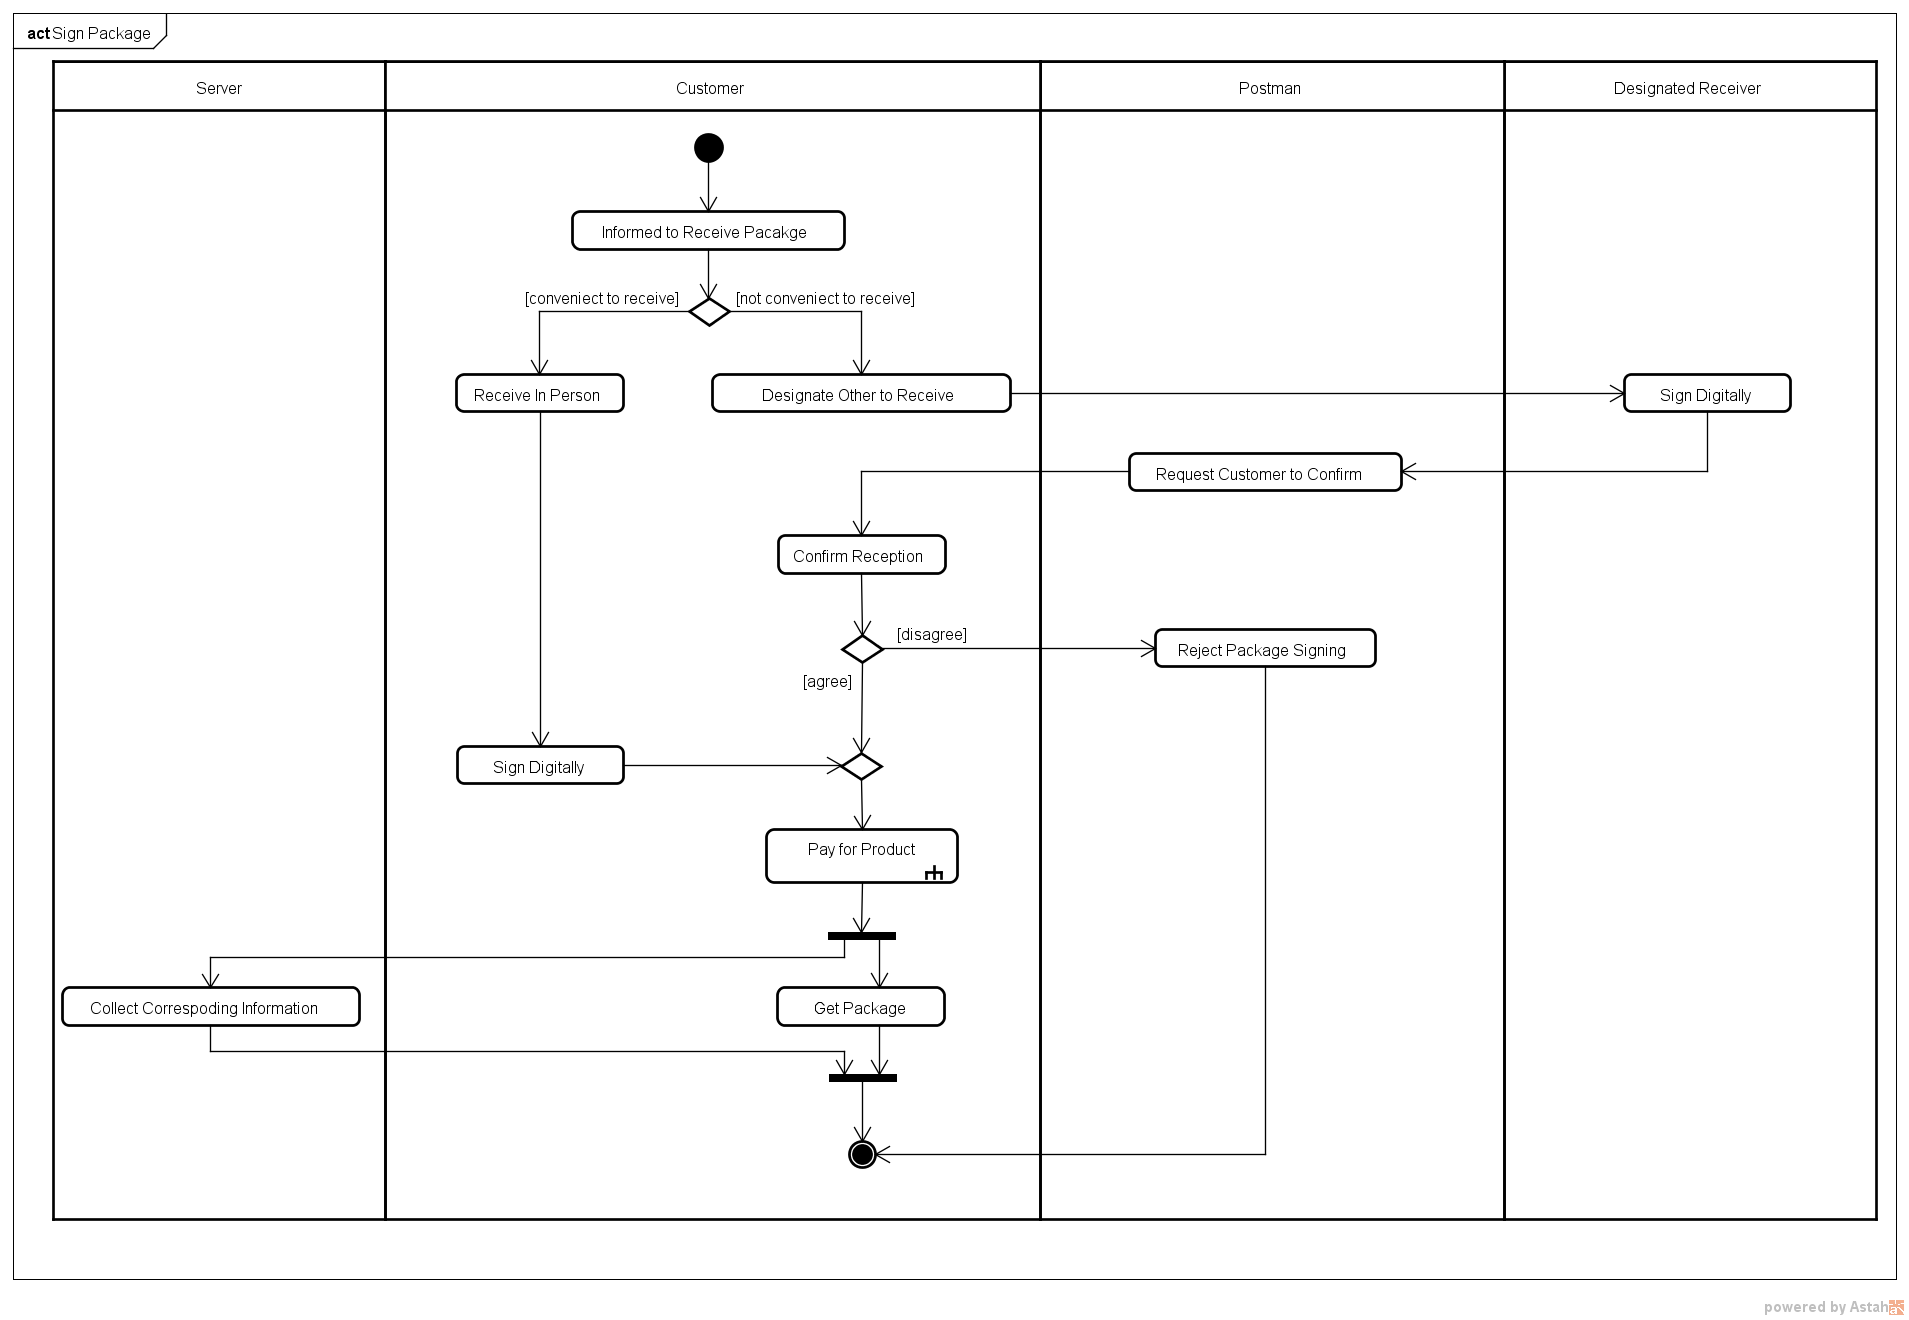
\includegraphics[width=5.5in]{DocumentRes/3SignPackage.png}
  \caption{Scenario Three Activity Diagram}
\end{figure}

\subsection{Scenario Four}
\begin{figure}[H]
  \centering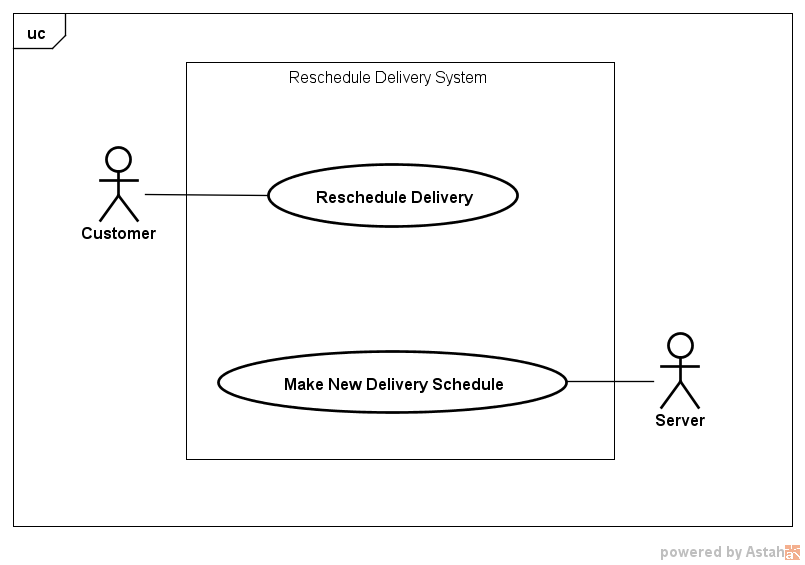
\includegraphics[width=4in]{DocumentRes/4UseCaseDiagram.png}
  \caption{Scenario Four Use Case Diagram}
\end{figure}

\begin{table}
  \centering
  \begin{tabular}{| c | p{11cm} |}
    \hline
    Use Case Name & Make New Delivery Schedule\\
    \hline
    Related Requirements & Scenario Four\\
    \hline
    Goal in Context & Rearrange package delivery.\\
    \hline
    Preconditions & No one receives the package.\\
    \hline
    Successful End Condition & A new delivery schedule is made; Parcel would
    be sent again.\\
    \hline
    Failed End Condition & Delivery reschedule failed.\\
    \hline
    Primary Actors & Server\\
    \hline
    Secondary Actors & Customer, Postman\\
    \hline
    Trigger & Server make a request of reschedule package delivery.\\
    \hline
    Main Flow & Step 1 : Server puts forward a new schedule.\\
    & Step 2 : Server sends the new plan to customer to see if customer is
    available then.\\
    & Step 3 : Customer replies yes.\\
    & Step 4 : Postman sends the package again according to new schedule that
    specified by customer.\\
    \hline
    Extensions & Step 3.1 : Customer replies no.\\
    & Step 3.2 : Made new delivery schedule again, or cancel the order.\\
    \hline
  \end{tabular}
\end{table}

\begin{table}
  \centering
  \begin{tabular}{| c | p{11cm} |}
    \hline
    Use Case Name & Reschedule Delivery\\
    \hline
    Related Requirements & Scenario Four\\
    \hline
    Goal in Context & Rearrange package delivery.\\
    \hline
    Preconditions & Customer does not receive the package.\\
    \hline
    Successful End Condition & A new delivery schedule is made; Parcel would
    be sent again.\\
    \hline
    Failed End Condition & Delivery reschedule failed.\\
    \hline
    Primary Actors & Customer\\
    \hline
    Secondary Actors & Server\\
    \hline
    Trigger & Customer requests to reschedule package delivery.\\
    \hline
    Main Flow & Step 1 : Customer requests the server to reschedule package
    delivery, sends a new time that he/she is available (and a new location if
    he/she needs).\\
    & Step 2 : Server makes a new delivery plan.\\
    & Include : Made New Delivery Schedule\\
    & Step 3 : Customer agrees.\\
    & Step 4 : New Schedule would be executed.\\
    \hline
    Extensions & Step 3.1 : Customer is not satisfied with the new schedule.\\
    & Step 3.2 : Made new delivery schedule again, or cancel the order.\\
    \hline
  \end{tabular}
\end{table}

\begin{table}
  \centering
  \begin{tabular}{| c | p{11cm} |}
    \hline
    Use Case Name & Report Delivery Failure\\
    \hline
    Related Requirements & Scenario Four\\
    \hline
    Goal in Context & Rearrange package delivery.\\
    \hline
    Preconditions & Customer does not receive the package.\\
    \hline
    Successful End Condition & A new delivery schedule is made; Parcel would
    be sent again.\\
    \hline
    Failed End Condition & Delivery reschedule failed.\\
    \hline
    Primary Actors & Postman\\
    \hline
    Secondary Actors & Server\\
    \hline
    Trigger & Package was received by no one.\\
    \hline
    Main Flow & Step 1 : Postman sends a report message, which inform the
    failure of delivery, to server.\\
    & Step 2 : Server makes a new delivery plan.\\
    & Include : Made New Delivery Schedule\\
    & Step 3 : A new feasible schedule is made, postman would execute it.\\
    \hline
    Extensions & Step 2.1 : Server fail to reschedule a new delivery plan.\\
    & Step 2.2 : Postman wait until a new delivery schedule is made, or the
    order is cancelled.\\
    \hline
  \end{tabular}
\end{table}

\begin{figure}[H]
  \centering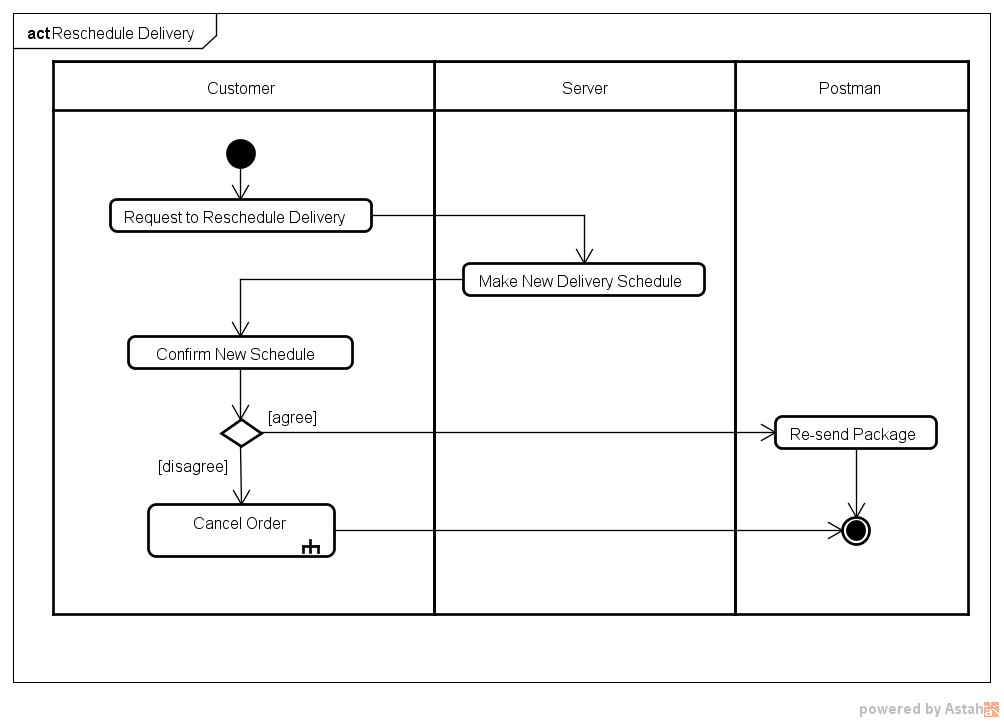
\includegraphics[width=5in]{DocumentRes/4RescheduleDelivery.png}
  \caption{Scenario Four Activity Diagram}
\end{figure}

\subsection{Scenario Five}
\begin{figure}[H]
  \centering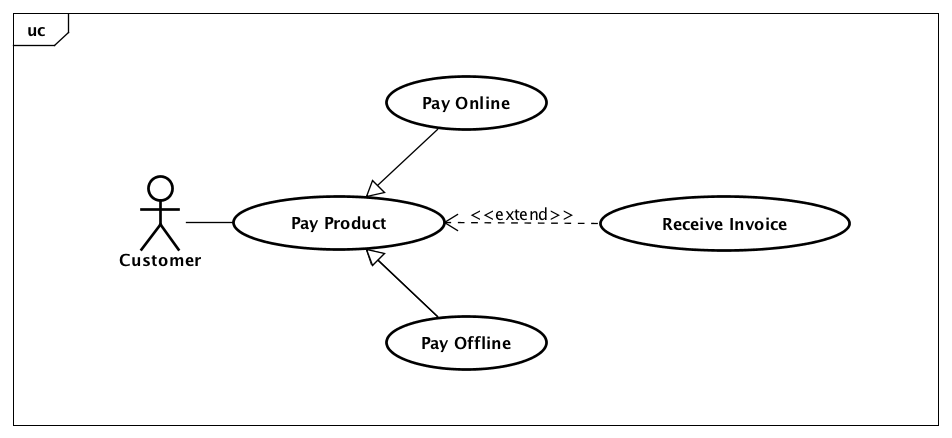
\includegraphics[width=4in]{DocumentRes/5UseCaseDiagram.png}
  \caption{Scenario Five Use Case Diagram}
\end{figure}

\begin{table}[H]
  \centering
  \begin{tabular}{| c | p{11cm} |}
    \hline
    Use Case Name & Pay for Product\\
    \hline
    Related Requirements & Scenario Five\\
    \hline
    Goal in Context & The customer needs to pay for the product after he/she
    has placed the product or received the product.\\
    \hline
    Preconditions & The customer has placed the order.\\
    \hline
    Successful End Condition & The payment is completed.\\
    \hline
    Failed End Condition & The order has been canceled or the customer has not
    received the product for some reasons.\\
    \hline
    Primary Actors & Customer\\
    \hline
    Secondary Actors & None\\
    \hline
    Trigger & The customer places the order or receives the product.\\
    \hline
    Main Flow & Step 1 : Customer chooses one acceptable way to pay for the
    product.\\
    & Step 2 : Customer checks the amount.\\
    & Step 3 : Customer finishes the payment.\\
    & Step 4 : E-business receives the payment.\\
    \hline
    Extensions & Step3.1 : Customer asks for a invoice about the product.\\
    \hline
  \end{tabular}
\end{table}

\begin{table}
  \centering
  \begin{tabular}{| c | p{11cm} |}
    \hline
    Use Case Name & Pay Online\\
    \hline
    Related Requirements & Scenario Five\\
    \hline
    Goal in Context & The customer wants to pay for the product online after
    he/she has placed the order.\\
    \hline
    Preconditions & The customer has placed the order, and paying online is
    provided.\\
    \hline
    Successful End Condition & The payment is completed.\\
    \hline
    Failed End Condition & The order has been canceled.\\
    \hline
    Primary Actors & Customer\\
    \hline
    Secondary Actors & None\\
    \hline
    Trigger & The customer places the order.\\
    \hline
    Main Flow & Step 1 : Customer logins the Third-party Trade system.\\
    & Step 2 : Customer checks the amount in the system.\\
    & Step 3 : Customer enters the passwords to pay.\\
    & Step 4 : Customer finishes the payment.\\
    & Step 5 : E-business receives the payment.\\
    \hline
    Extensions & None\\
    \hline
  \end{tabular}
\end{table}

\begin{table}
  \centering
  \begin{tabular}{| c | p{11cm} |}
    \hline
    Use Case Name & Pay Offline\\
    \hline
    Related Requirements & Scenario Five\\
    \hline
    Goal in Context & The customer wants to pay for the product offline after
    he/she has received the product.\\
    \hline
    Preconditions & The customer has received the product, and paying offline
    is provided.\\
    \hline
    Successful End Condition & The payment is completed.\\
    \hline
    Failed End Condition & The customer has not received the product for some
    reasons.\\
    \hline
    Primary Actors & Customer\\
    \hline
    Secondary Actors & Postman\\
    \hline
    Trigger & The customer receives the product.\\
    \hline
    Main Flow & Step 1 : Postman checks the amount with the customer.\\
    & Step 2 : Customer chooses one way to pay, by cash or by credit card.\\
    & Step 3 : Customer finishes the payment.\\
    & Step 4 : Postman records the information about the payment.\\
    & Step 5 : The logistics company transfers the money to E-business.\\
    \hline
    Extensions & Step 2.1 : Customer chooses to pay by cash.\\
    & \ \ Customers pays for the product by cash.\\
    & \ \ Postman checks the amounts of money and confirms the payment in the app.\\
    & Step 2.2 : Customer Chooses to pay by credit card.\\
    & \ \ Postman provide the POS device for the customer.\\
    & \ \ Customer gives the postman his/her Visa card or Union-Pay card.\\
    & \ \ Postman swipes the card and enters the amount of money.\\
    & \ \ Customer enters the password.\\
    & \ \ The bank system adds money to the logistics company’s account.\\
    & Step 4.1 : Postman submits the money to the logistics company.\\
    \hline
  \end{tabular}
\end{table}

\begin{table}[H]
  \centering
  \begin{tabular}{| c | p{11cm} |}
    \hline
    Use Case Name & Provide Invoice\\
    \hline
    Related Requirements & Scenario Five\\
    \hline
    Goal in Context & E-business provides the invoice about the product for
    the customer.\\
    \hline
    Preconditions & The customer has completed the payment and asks for
    the invoice.\\
    \hline
    Successful End Condition & The Invoice has been sent to the customer.\\
    \hline
    Failed End Condition & E-business rejects the request.\\
    \hline
    Primary Actors & E-business\\
    \hline
    Secondary Actors & Customer\\
    \hline
    Trigger & Customer asks for the invoice about the product.\\
    \hline
    Main Flow & Step 1 : Customer choose one way to receive the invoice,
    digital invoice sent by e-mail or a paper invoice sent by post.\\
    & Step 2 : E-business sends the invoice to the customer.\\
    & Step 3 : Customer receives the invoice and confirm whether
    the infomation is onsistent.\\
    \hline
    Extensions & Step 1.1 : Customer chooses to receive a digital invoice
    sent by e-mail.\\
    & \ \ Customer fills in the e-mail address in the app.\\
    & Step 1.2 : Customer chooses to receive a paper invoice sent by post.\\
    & \ \ Customer fills in the mailing address in the app.\\
    \hline
  \end{tabular}
\end{table}

\begin{figure}[H]
  \centering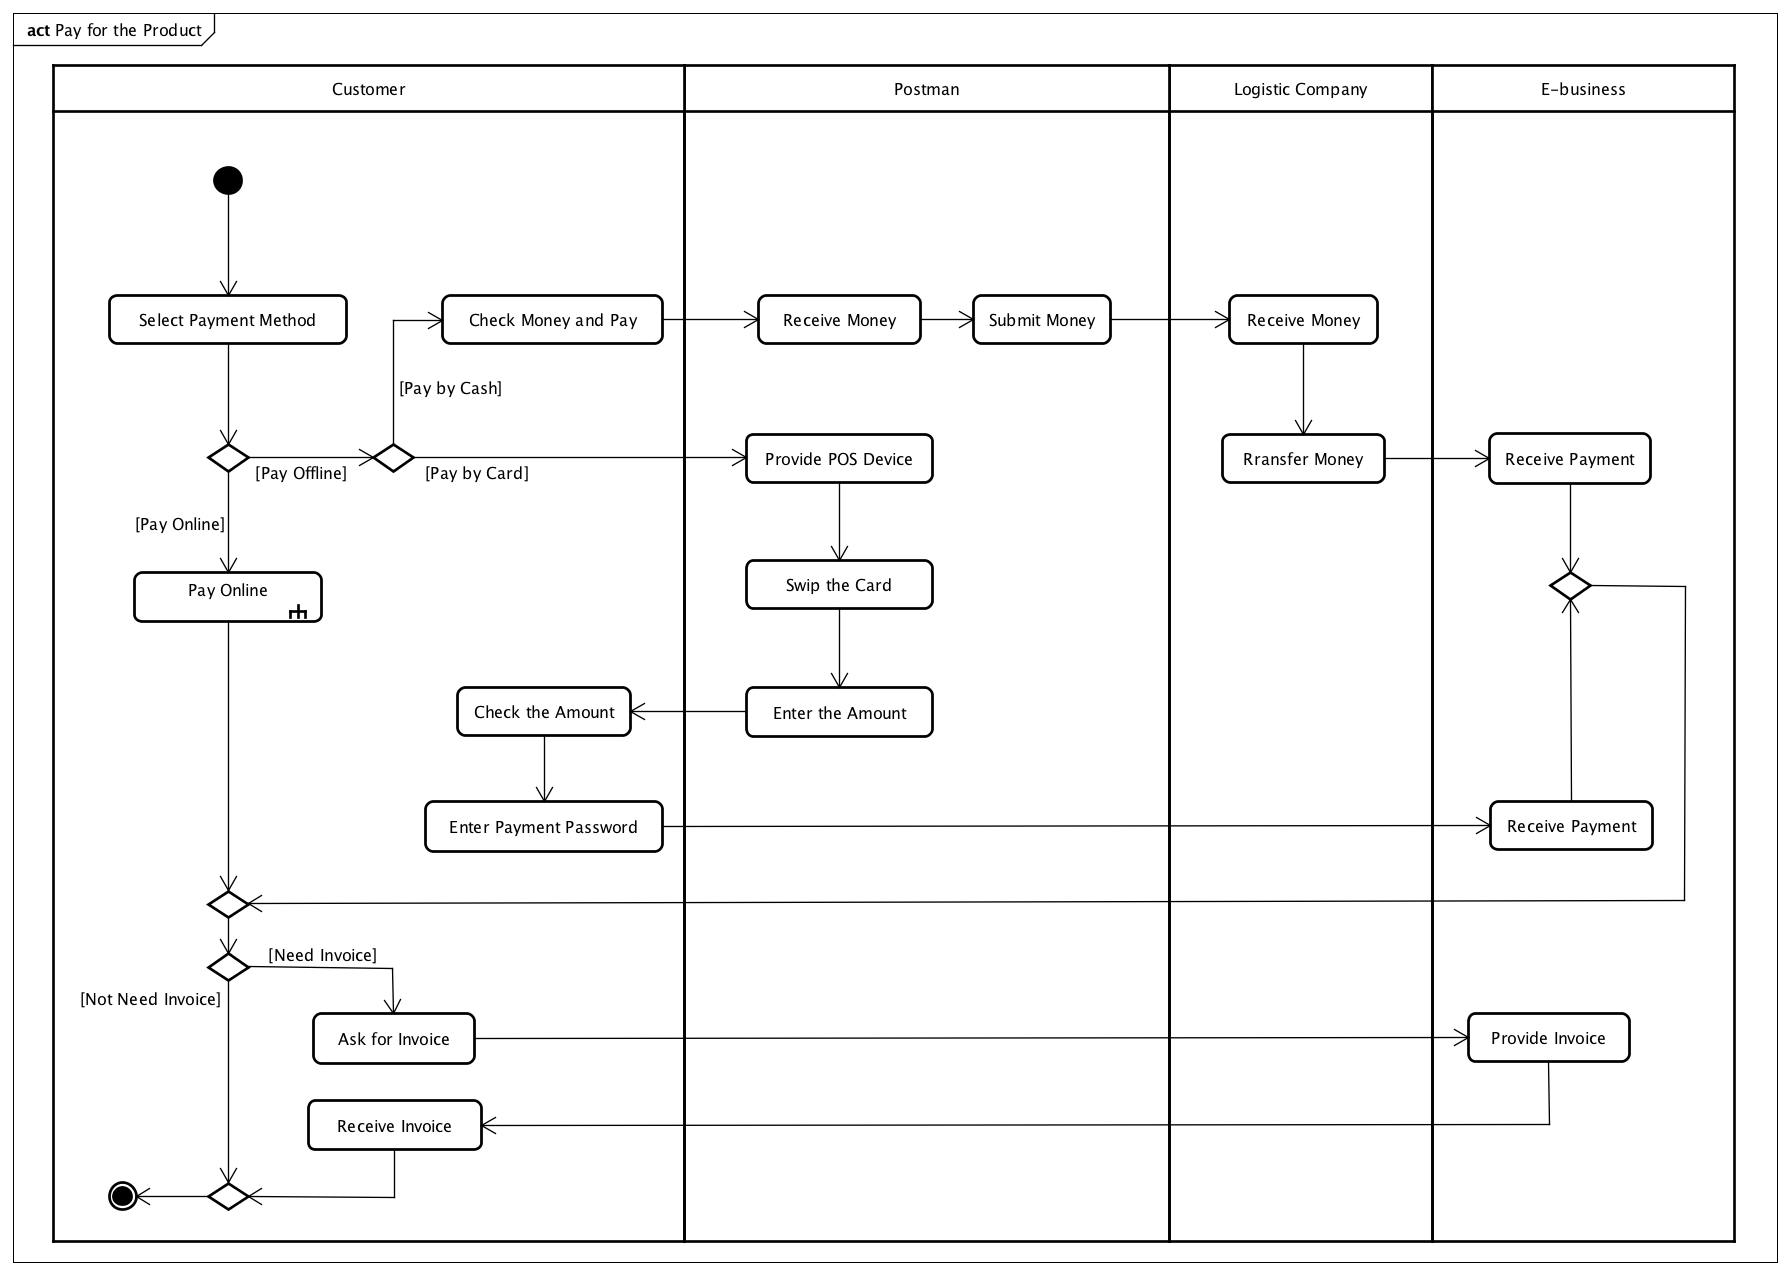
\includegraphics[width=5in]{DocumentRes/5PayTheProduct.png}
  \caption{Scenario Five Activity Diagram: Pay The Product}
\end{figure}

\begin{figure}[H]
  \centering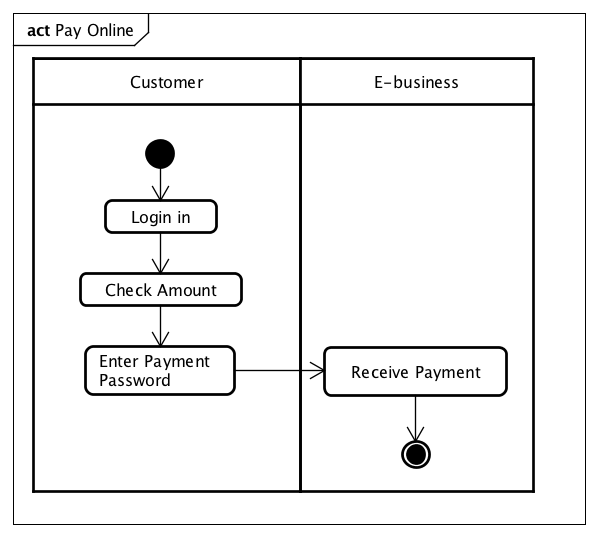
\includegraphics[width=3.5in]{DocumentRes/5PayOnline.png}
  \caption{Scenario Five Activity Diagram: Pay Online}
\end{figure}

\subsection{Scenario Six}
\begin{figure}[H]
  \centering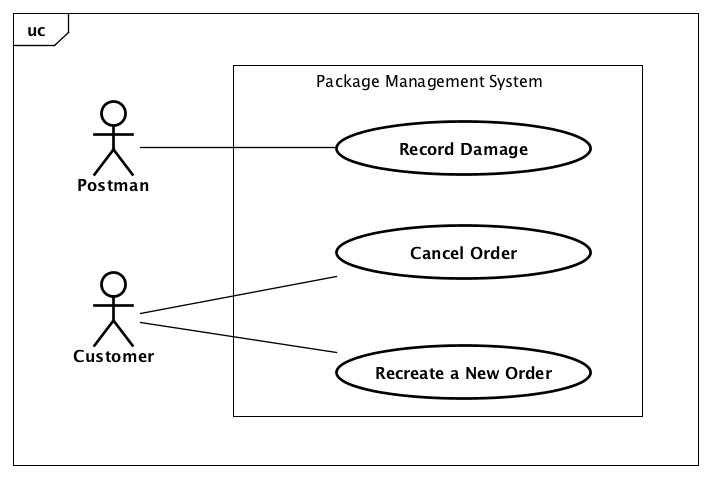
\includegraphics[width=4in]{DocumentRes/6UseCaseDiagram.png}
  \caption{Scenario Six Use Case Diagram}
\end{figure}

\begin{table}[H]
  \centering
  \begin{tabular}{| c | p{11cm} |}
    \hline
    Use Case Name & Record Damage\\
    \hline
    Related Requirements & Scenario Six\\
    \hline
    Goal in Context & Postman records the information of the damaged or
    lost package.\\
    \hline
    Preconditions & The package was damaged or lost.\\
    \hline
    Successful End Condition & Postman records the infomation successfully.\\
    \hline
    Failed End Condition & The information of the package was lost as well.\\
    \hline
    Primary Actors & Postman\\
    \hline
    Secondary Actors & None\\
    \hline
    Trigger & The package was damaged or lost.\\
    \hline
    Main Flow & Step 1 : Postman records the information of the package.\\
    & Step 2 : The logistics company receives the corresponding information.\\
    & Step 3 : The logistics company sends a message to the customer,
    explaining the situation and making an apology to the customer.\\
    \hline
    Extensions & None\\
    \hline
  \end{tabular}
\end{table}

\begin{table}
  \centering
  \begin{tabular}{| c | p{11cm} |}
    \hline
    Use Case Name & Cancel Order\\
    \hline
    Related Requirements & Scenario Six\\
    \hline
    Goal in Context & The customer wants to cancel the order for some reasons.\\
    \hline
    Preconditions & The customer has placed the order. The package has not
    been shipped or the package was damaged or lost during process of delivery.\\
    \hline
    Successful End Condition & The logistics company passes the request.\\
    \hline
    Failed End Condition & The request is rejected.\\
    \hline
    Primary Actors & Customer\\
    \hline
    Secondary Actors & None\\
    \hline
    Trigger & The customer makes the request of canceling the order.\\
    \hline
    Main Flow & Step 1 : Customer logins the logistics system.\\
    & Step 2 : Customer selects the button "cancel the order".\\
    & Step 3 : Customer explains the reason.\\
    & Step 4 : The logistics company receives the request and passes the
    request.\\
    \hline
    Extensions & None\\
    \hline
  \end{tabular}
\end{table}

\begin{table}
  \centering
  \begin{tabular}{| c | p{11cm} |}
    \hline
    Use Case Name & Recreate a New Order\\
    \hline
    Related Requirements & Scenario Six\\
    \hline
    Goal in Context & The customer wants to recreate a new order without any
    extra fees beceause the old package was damaged or lost.\\
    \hline
    Preconditions & The old package was damaged or lost and the customer has
    eceived the message from the logistics company.\\
    \hline
    Successful End Condition & The new order is placed successfully.\\
    \hline
    Failed End Condition & The new order is non-compliant and rejected.\\
    \hline
    Primary Actors & Customer\\
    \hline
    Secondary Actors & None\\
    \hline
    Trigger & The customer makes the request of recreating a new order.\\
    \hline
    Main Flow & Step 1 : Customer receives the message about the infomation
    of the damaged or lost package.\\
    & Step 2 : Customer logins the logistics system.\\
    & Step 3 : Customer chooses to deliver a new package.\\
    & Step 4 : Customer fills in the basic information and recreates a new
    order whithout any extra fees.\\
    & Step 5 : The logistics company receives the new order and passes
    the request.\\
    \hline
    Extensions & None\\
    \hline
  \end{tabular}
\end{table}

\begin{figure}[H]
  \centering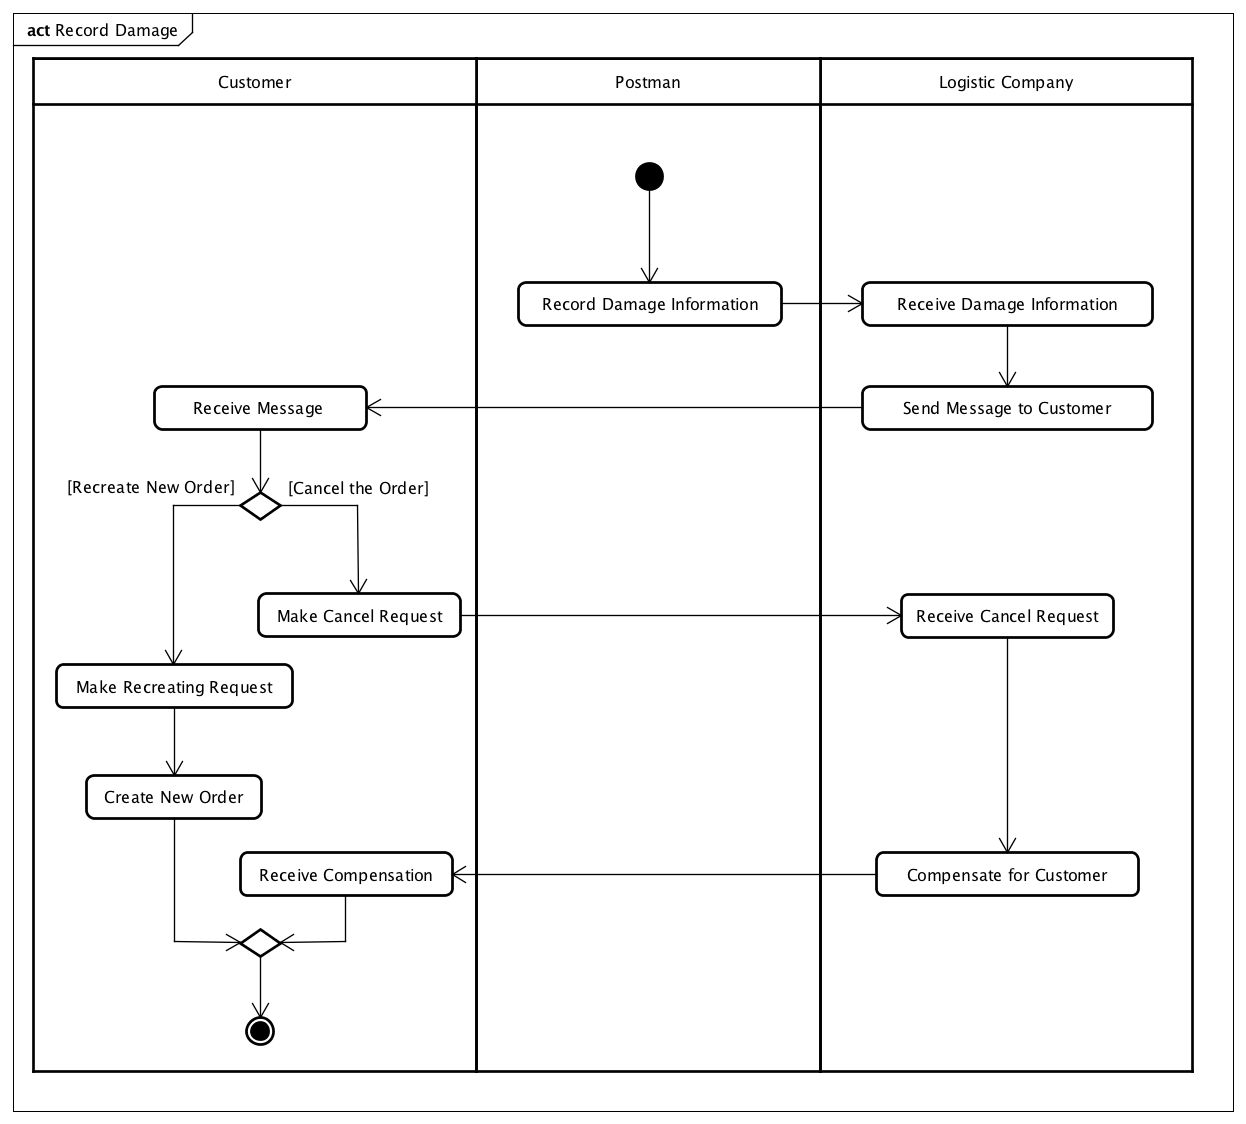
\includegraphics[width=6in]{DocumentRes/6RecordDamage.png}
  \caption{Scenario Six Activity Diagram}
\end{figure}

\subsection{Scenario Seven}
\begin{figure}[H]
  \centering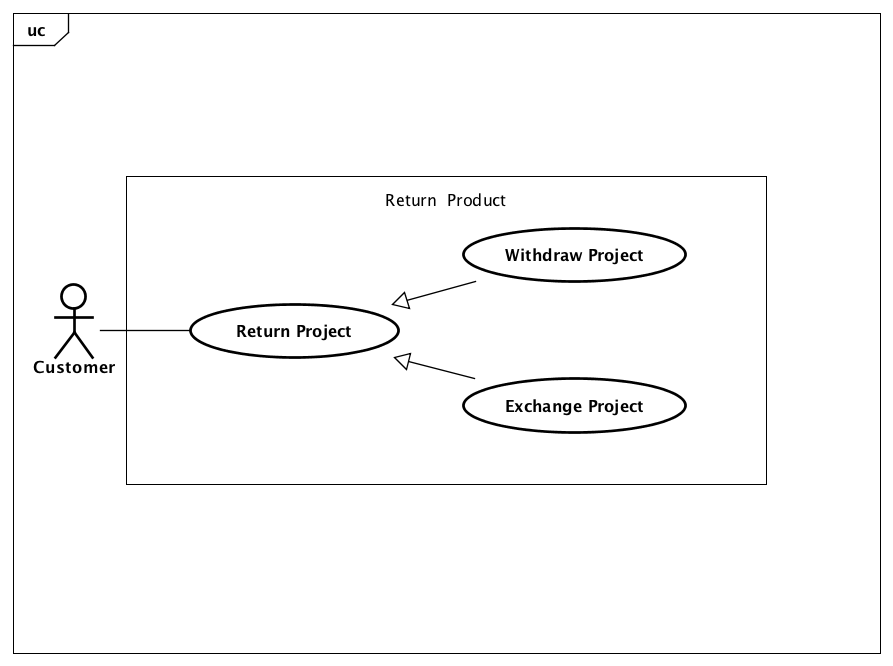
\includegraphics[width=3.5in]{DocumentRes/7UseCaseDiagram.png}
  \caption{Scenario Seven Use Case Diagram}
\end{figure}

\begin{table}[H]
  \centering
  \begin{tabular}{| c | p{11cm} |}
    \hline
    Use Case Name & Withdraw Product\\
    \hline
    Related Requirements & Scenario Seven\\
    \hline
    Goal in Context & A customer returns the product and the payment is
    reimbursed.\\
    \hline
    Preconditions & The customer wants to withdraw the product the or she
    unsatisfied with after receiving within a month.\\
    \hline
    Successful End Condition & The order is completed and the payment is
    reimbursed to the customer.\\
    \hline
    Failed End Condition & The order is not completed and the payment is not
    reimbursed to the customer.\\
    \hline
    Primary Actors & Customer\\
    \hline
    Secondary Actors & None\\
    \hline
    Trigger & The customer choose to withdraw the product.\\
    \hline
    Main Flow & Step 1 : Customer makes the returning request.\\
    & Step 2 : Server checks the returning request.\\
    & Step 3 : The package is delivered.\\
    & Step 4 : The E-business receives and checks the pack.\\
    & Step 5 : The E-business agrees the returning.\\
    & Step 6 : Server make the new delivery schedule.\\
    \hline
    Extensions & Step 2.1 : The database does not verify the details.\\
    & Step 3.1 : The package fails to be delivered.\\
    & Step 5.1 : The E-business doesn't agree the withdrawing.\\
    \hline
  \end{tabular}
\end{table}

\begin{table}
  \centering
  \begin{tabular}{| c | p{11cm} |}
    \hline
    Use Case Name & Exchange Product\\
    \hline
    Related Requirements & Scenario Seven\\
    \hline
    Goal in Context & A customer returns the product and the delivery schedule
    is made again upon mutual agreement.\\
    \hline
    Preconditions & The customer wants to exchange the product the or she
    unsatisfied with after receiving within a month.\\
    \hline
    Successful End Condition & The delivery schedule is made again upon
    mutual agreement.\\
    \hline
    Failed End Condition & The delivery schedule fails to be made again upon
    mutual agreement.\\
    \hline
    Primary Actors & Customer\\
    \hline
    Secondary Actors & None\\
    \hline
    Trigger & The customer choose to exchange the product.\\
    \hline
    Main Flow & Step 1 : Customer makes the returning request.\\
    & Step 2 : Server checks the returning request.\\
    & Step 3 : The package is delivered.\\
    & Step 4 : The E-business receives and checks the pack.\\
    & Step 5 : The E-business agrees the returning.\\
    & Step 6 : Server make the new delivery schedule.\\
    \hline
    Extensions & Step 2.1 : The database does not verify the details.\\
    & Step 3.1 : The package fails to be delivered.\\
    & Step 5.1 : The E-business doesn't agree the exchange.\\
    \hline
  \end{tabular}
\end{table}

\begin{figure}[H]
  \centering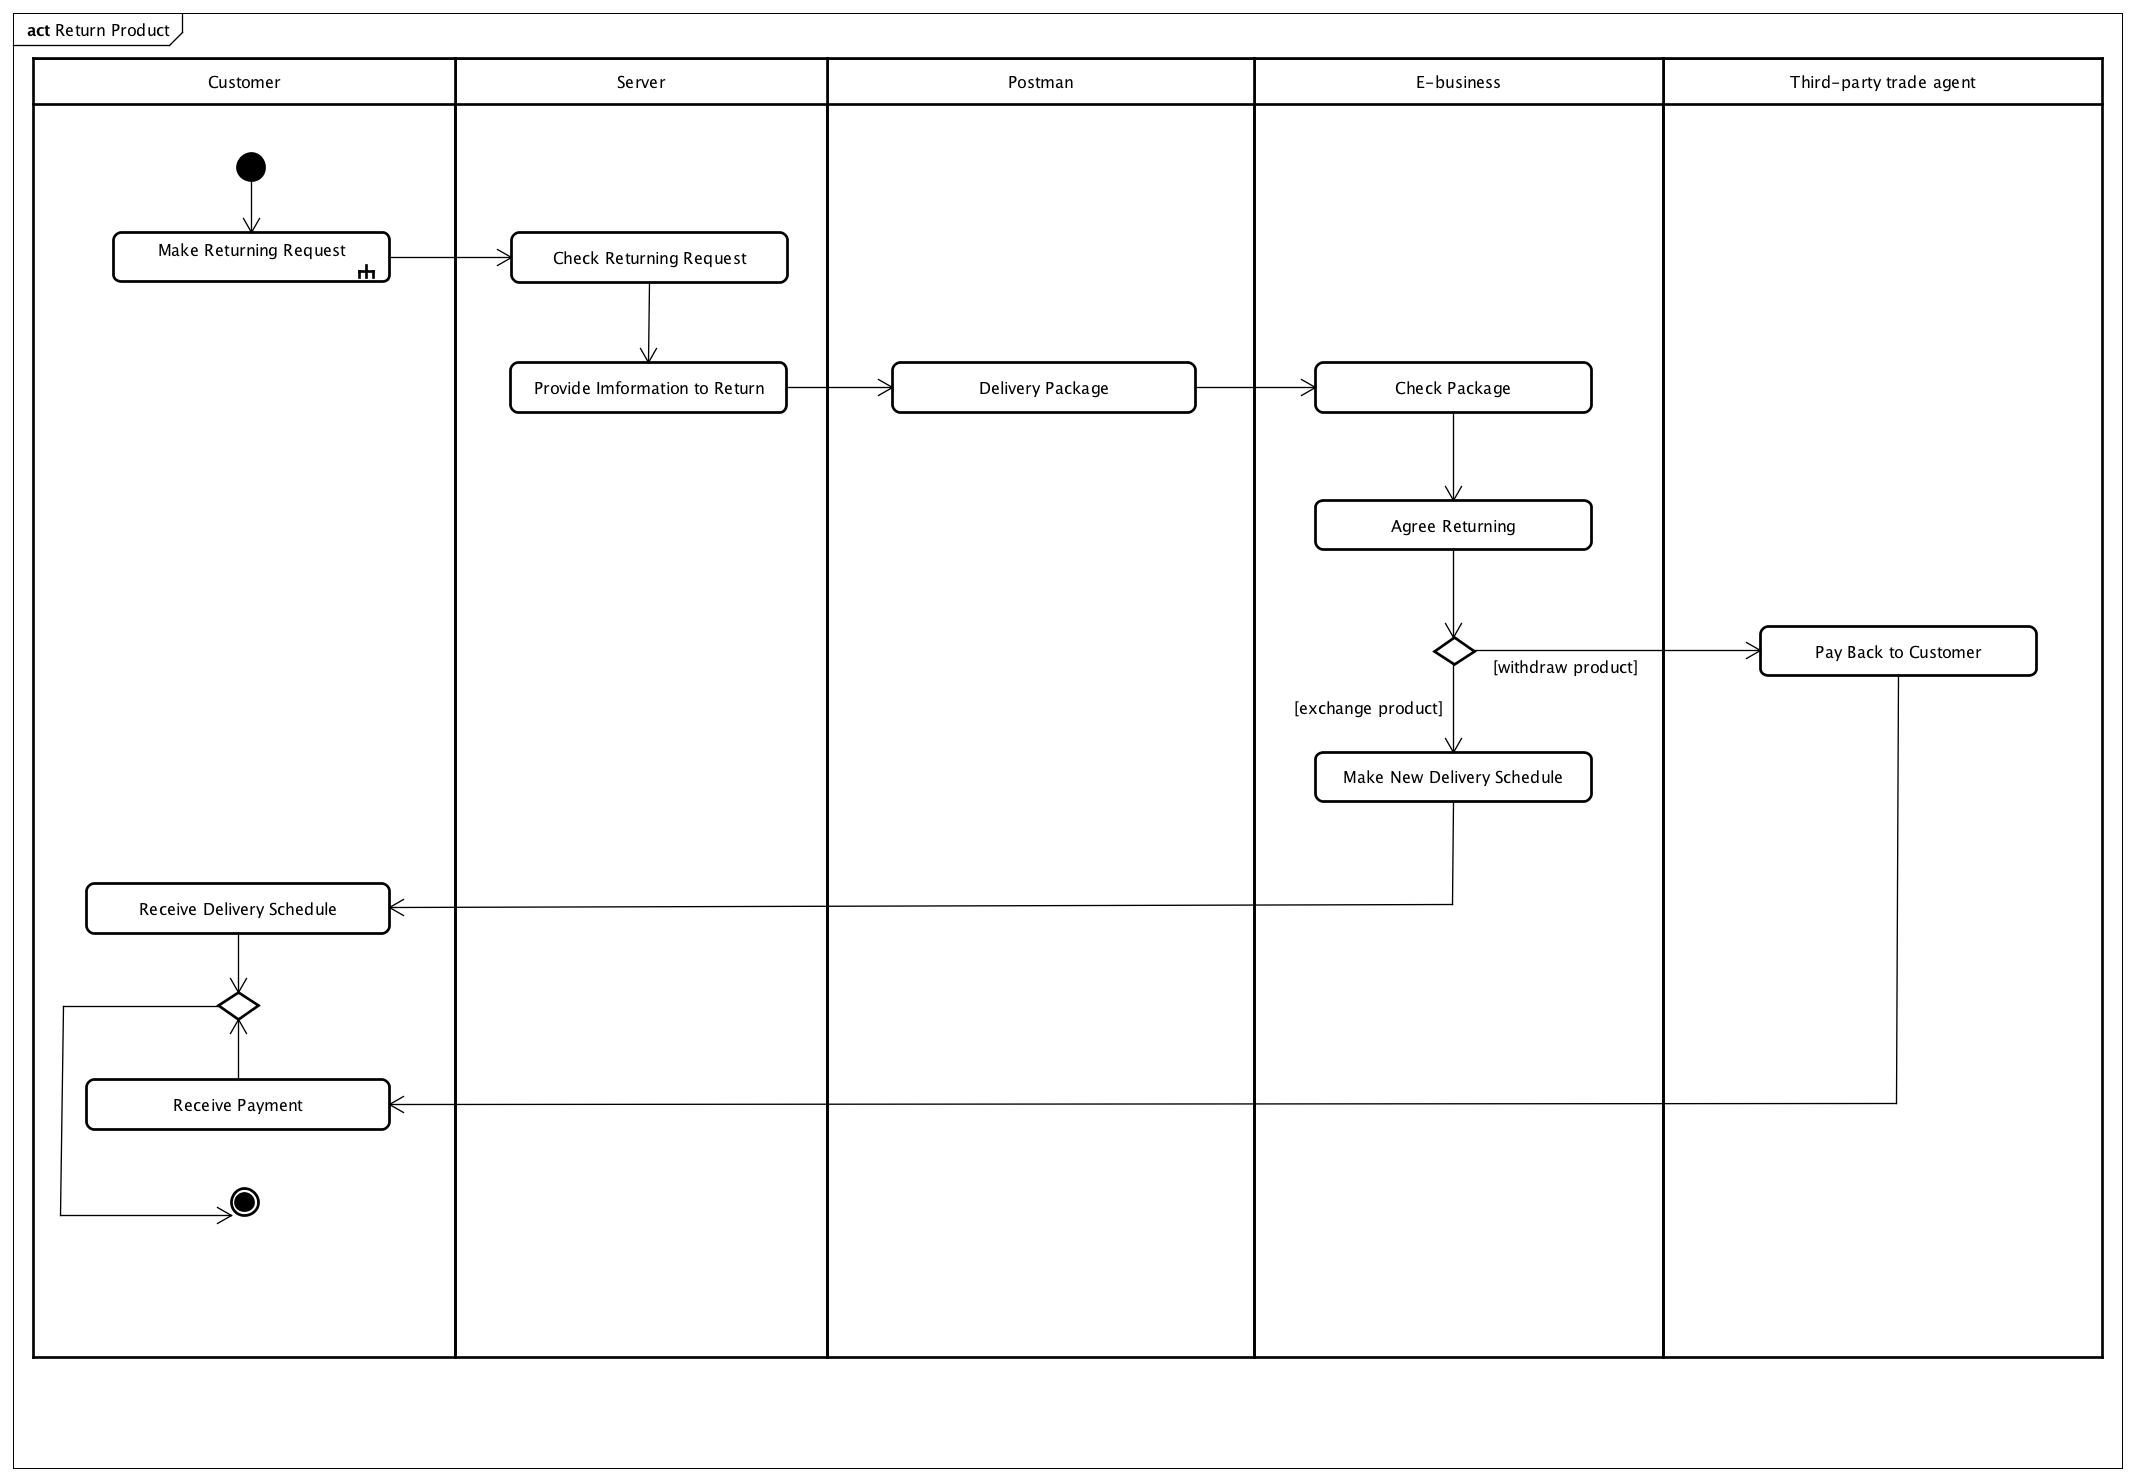
\includegraphics[width=6in]{DocumentRes/7ReturnProduct.png}
  \caption{Scenario Seven Activity Diagram: Return Product}
\end{figure}

\begin{figure}[H]
  \centering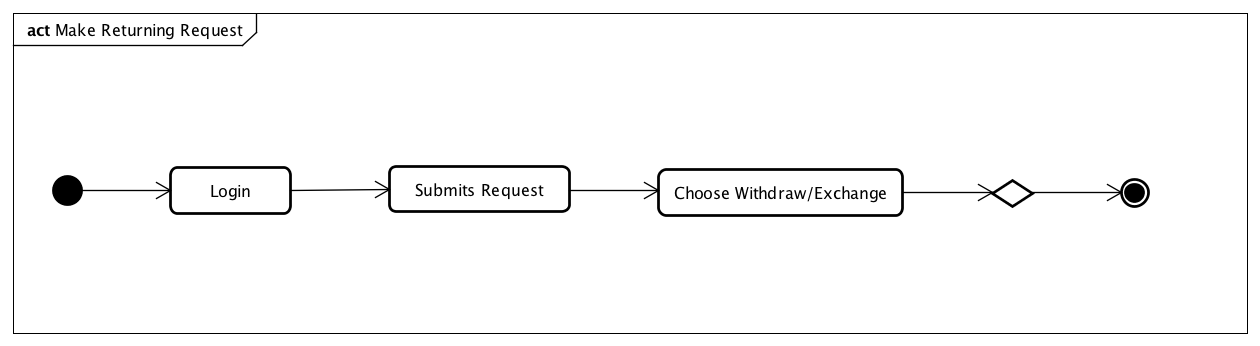
\includegraphics[width=5in]{DocumentRes/7MakeReturningRequest.png}
  \caption{Scenario Seven Activity Diagram: Make Returning Request}
\end{figure}

\subsection{Scenario Eight}
\begin{figure}[H]
  \centering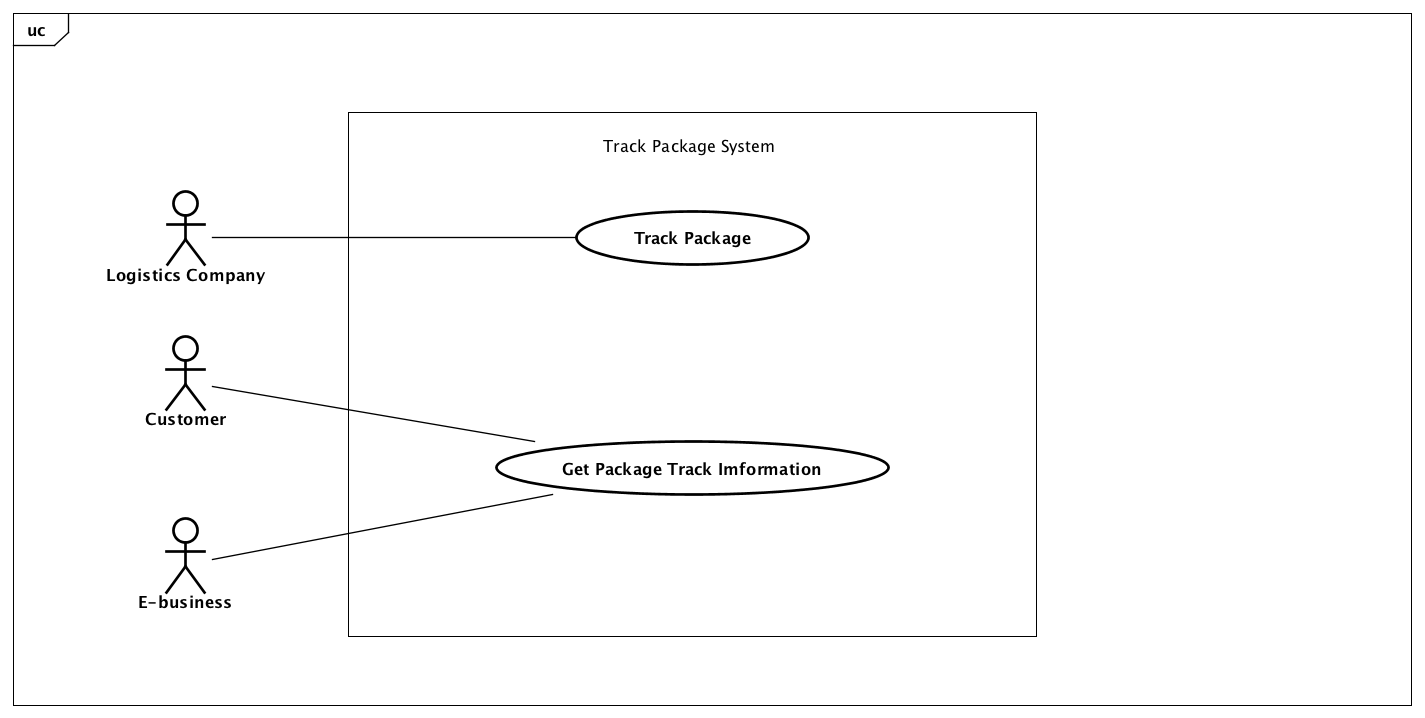
\includegraphics[width=4in]{DocumentRes/8UseCaseDiagram.png}
  \caption{Scenario Seven Use Case Diagram}
\end{figure}

\begin{table}[H]
  \centering
  \begin{tabular}{| c | p{11cm} |}
    \hline
    Use Case Name & Track Package\\
    \hline
    Related Requirements & Scenario Eight\\
    \hline
    Goal in Context & The logistics tracks all the packages, collecting the
    location at fixed period and inserting new addresses of destinations into
    the database.\\
    \hline
    Preconditions & The customer or the e-business company deliver the package.\\
    \hline
    Successful End Condition & The logistics tracks all the packages and feeds
    back to the customer or the E-business.\\
    \hline
    Failed End Condition & The logistics fails track all the packages and feed
    back to the customer or the E-business.\\
    \hline
    Primary Actors & Logistics\\
    \hline
    Secondary Actors & None\\
    \hline
    Trigger & Postman receives the package from the customer.\\
    \hline
    Main Flow & Step 1 : Postman receives and expresses the package to the
    logistics.\\
    & Step 2 : Logistics delivers the package to the express station.\\
    & Step 3 : The express station  scans the bar code.\\
    & Step 4 : Server records the express station information of the package.\\
    & Step 5 : Logistics delivers the package to the next express station.\\
    \hline
    Extensions & Step 3.1 : The express station fails to scan the bar code
    and gets a new bar code.\\
    \hline
  \end{tabular}
\end{table}

\begin{table}
  \centering
  \begin{tabular}{| c | p{11cm} |}
    \hline
    Use Case Name & Get Package Track Inmformation\\
    \hline
    Related Requirements & Scenario Eight\\
    \hline
    Goal in Context & The customer or the e-business can get track Inmformation
    of the package delivered.\\
    \hline
    Preconditions & 1. The returning request is admitted.\\
    & 2. The customer or E-business delivers the returning product.\\
    & 3. The package has not been transferred to the receiver.\\
    & 4.The customer or the E-business has obtained the tracking number.\\
    & 5.The logistics tracks all the packages, collecting the GPS location at
    fixed period and inserting new GPS addresses of destinations into the
    database automatically.\\
    \hline
    Successful End Condition & The customer or the e-business successfully
    tracks the package he or she delivered.\\
    \hline
    Failed End Condition & The customer or the e-business successfully failed
    to track the package he or she delivered.\\
    \hline
    Primary Actors & Customer, E-business\\
    \hline
    Secondary Actors & None\\
    \hline
    Trigger & The customer or the E-business logins the system.\\
    \hline
    Main Flow & Step 1 : The customer or the E-business logins the system.\\
    & Step 2 : The customer or the E-business inputs the tracking number.\\
    & Step 3 : The customer or the E-business get package track information.\\
    \hline
    Extensions & Step 1.1 : The customer or the E-business failed to login the
    system with the wrong account and password.\\
    \hline
  \end{tabular}
\end{table}

\begin{figure}[H]
  \centering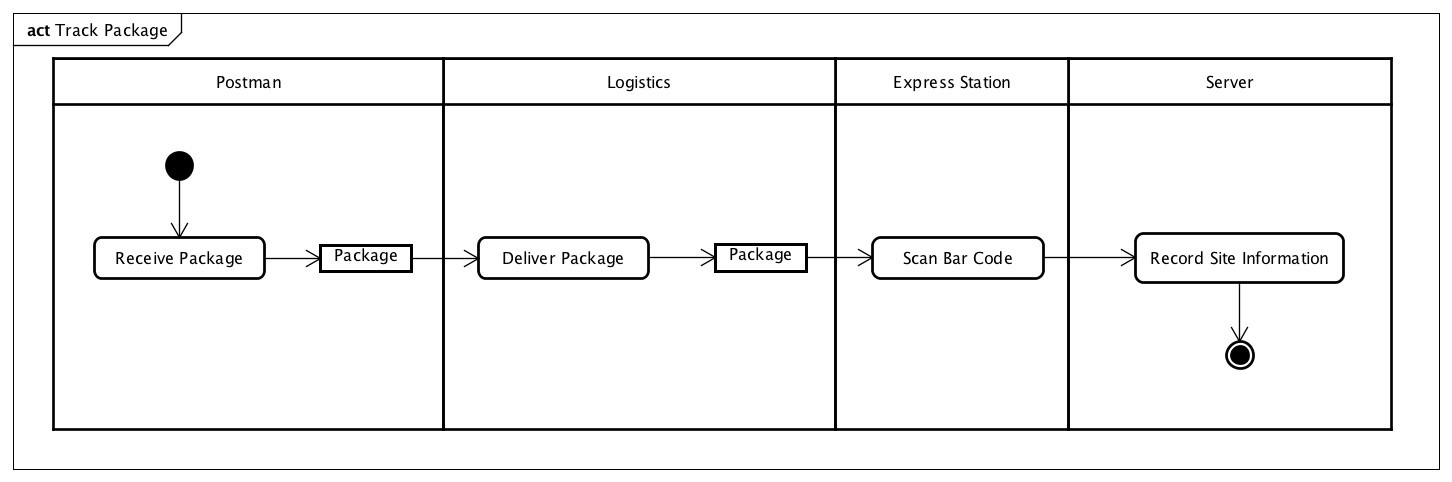
\includegraphics[width=5in]{DocumentRes/8TrackPackage.png}
  \caption{Scenario Seven Activity Diagram: Track Package}
\end{figure}

\begin{figure}[H]
  \centering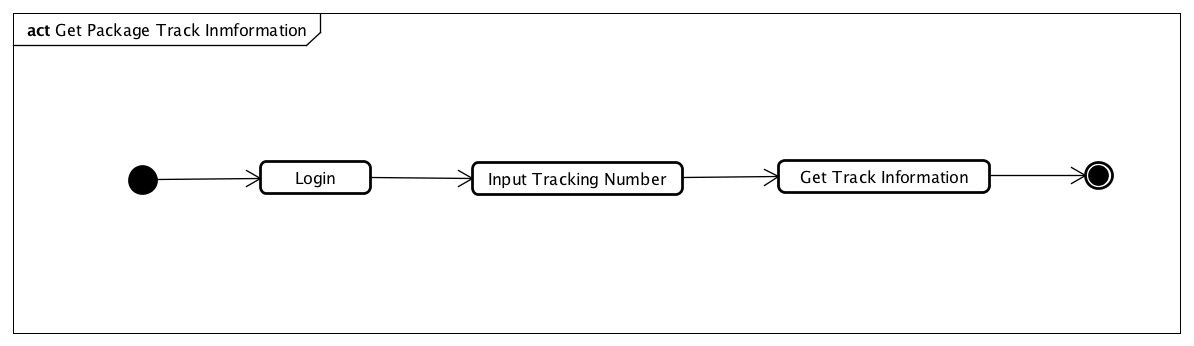
\includegraphics[width=5in]{DocumentRes/8GetPackageTrackInmformation.png}
  \caption{Scenario Seven Activity Diagram: Get Package Track Inmformation}
\end{figure}

\chapter{Glossary of Terms}
\begin{spacing}{0.7}
\subsubsection{after-sales service}
Also called customer service, after sales service is the provision of
service to customers before, during and after a purchase.
\subsubsection{article}
The material in the package which is sent by a normal customer.
\subsubsection{bi-directional read}
The information can be read in both direction.
\subsubsection{cash-on-delivery express}
The sale of goods by express where payment is made on delivery rather
than in advance.
\subsubsection{claim}
When packages are damaged or lost, customers have right to ask for compensation.
\subsubsection{courier}
A courier is a person who delivers messages, packages, and mail. Here it refers
to postmen.
\subsubsection{customer service staff}
The staff in the logistics company serving customers.
\subsubsection{damaged express item}
The package that is damaged during express.
\subsubsection{decision support system(DSS)}
A decision support system is a computer-based information system that supports
 business or organizational decision-making activities.
\subsubsection{delivery}
A single task to send the package to a customer.
\subsubsection{delivery terminal}
The destination of the delivery where the receiver receive and sign the package.
\subsubsection{dispath list}
The digital list of information of the packages to be delivered in
postmen’s port.
\subsubsection{distribution center}
A station in a large district to transfer packages to the regional
distribution center.
\subsubsection{door-to-cfs}
From the shipper factory or warehouse to the destination or the
Container freight station of the discharging port.
\subsubsection{door-to-door}
From the shipper factory or warehouse to the consignee's factory
or warehouse.
\subsubsection{Electronic Data Interchange(EDI)}
Electronic Data Interchange is an electronic communication method that provides
standards for exchanging data via any electronic means.
\subsubsection{Electronic Order System(EOS)}
Electronic Order System is to meet demand instantly,
with perfect quality and punctuality.
\subsubsection{express item}
Packages to be delivered.
\subsubsection{express item tracking system}
A subsystem in our system to track the packages with GIS automatically.
\subsubsection{express network}
A service network within the scope to help delivery.
\subsubsection{express waybill}
An express receipt given by the carrier to the shipper acknowledging receipt
of the packages being shipped and specifying the terms of delivery.
\subsubsection{first time delivery}
The first time for particular postman to send the package to a position.
\subsubsection{Global Position System(GPS)}
The Global Positioning System is a space-based navigation system that
provides location and time information in all weather conditions,
anywhere on or near the Earth where there is an unobstructed line of
sight to four or more GPS satellites.
\subsubsection{Geographic Information System(GIS)}
A geographic information system is a system designed to capture,
store, manipulate, analyze, manage, and present all types of spatial
or geographical data.
\subsubsection{handheld terminal}
Handheld terminal refers to the portable data processing terminal
with some particular features. Here it refers to mobile phones with our app.
\subsubsection{inquiry}
The customer logins the system or connects with customer service staff to get
information about the order, operation instruction etc.
\subsubsection{Integrated Services Digital Network(ISDN)}
Integrated Services for Digital Network is a set of communication standards
for simultaneous digital transmission of voice, video, data, and other
network services over the traditional circuits of the public switched
telephone network.
\subsubsection{interchange receipt}
A voucher to certify that the customers or e-business commits articles
or products to the logistics company for delivery.
\subsubsection{Invoice(INV)}
An invoice is a commercial document issued by a seller to a buyer,
relating to a sale transaction and indicating the products, quantities,
and agreed prices for products or services the seller had provided the buyer.
\subsubsection{Just-in-time logistics(JIT logistics)}
Just-in-time logistics is a modern logistics method based on the JIT
management philosophy.
\subsubsection{lost express item}
The package that is lost during express.
\subsubsection{order number}
The number generalized when the order is created.
\subsubsection{order processing}
A series automatic operation in system to deal the order, such as
creating an order, completing an order and so on.
\subsubsection{package}
The material to be delivered after customers or the e-business company
create orders.
\subsubsection{product}
The material in the package which is ordered by customers from the
e-business company.
\subsubsection{receiver}
Generalized from Customer and Agent, the person receiving and signing
the package directly.
\subsubsection{redelivery}
When no one can sign the package, the postman will carry it back to
the delivery terminal and the order will be rescheduled in the system.
\subsubsection{redirect express item}
When customer changes the destination or the destination is out of scope,
the package will be reassigned.
\subsubsection{regional distribution center}
The substation in a certain region of the logistics company to assign
packages to postmen.
\subsubsection{return}
If customers are unsatisfied with the product, he or she can send it back
with a label from system.
\subsubsection{sender}
The customer or the e-business company who sends the package.
\subsubsection{serial number of express}
i.e. the tracking number of packages in the system.
\subsubsection{sign in}
The receiver sign the package and get it.
\subsubsection{sorting}
The packages in the regional distribution center are sorted to transfer to
corresponding postmen or the packages in the distribution center are sorted to
transport to regional distribution centers.
\subsubsection{tracking number}
Especially for tracking the real-time GPS location of the package.
\subsubsection{withdrawal}
If the customer is unsatisfied with the product and has sent it back,
he or she can choose withdraw the order and the payment will be reimbursed.
\end{spacing}

\chapter{Supplementary Specification}
\section{Security}
The system should avoid the database being attacked and data being taken
advantage of by the wicked.
\subsection{Access and Data Integrity}
\begin{enumerate}
  \item The authorization of access to the system of postmen, customers
  and customer servers should be classified and announced clearly. With
  certain authorization, different users have limited access to data and
  operation.
  \item The server should use anti-virus software.
  \item Firewalls and network protection are necessary, and they should
  be updated in time.
  \item The atomic processes in the database will ensure the accuracy
  of the database.
\end{enumerate}

\subsection{Encryption}
\begin{enumerate}
  \item The session should not be transmitted in DNS.
  \item All texts and messages should be encrypted with Encryption Algorithm
  such as RSA, 3DES or IDEA.
  \item Two keys are used to identify a certain user. One public key is
  used for encryption and anther private key is used for decryption.
  The key is a completely random mix of letters.
  \item The session will record the activity of the customer, and if the
  customer has no operation for 5 minutes, he or she will log out the system
  automatically.
  \item After customers log out the system, all the private information(cookies)
  will be cleaned.
\end{enumerate}

\subsection{Digital Certificates}
\begin{enumerate}
  \item We use digital certificates as a replacement of user names and
  passwords, for example, SSL Certificates. It will be used automatically
  with the permission of users.
  \item The IP address or location where users log in the system will be
  recorded and when the account is used beyond their regular locations, the
  user will get alarmed.
\end{enumerate}

\subsection{Digital Signatures}
\begin{enumerate}
  \item Users should log in the system with a password. Our system will
  test its complexity. If it is too simple, the system will remind the
  users to complicate it. That involves cryptography.
  \item We use a message digest to ensure the integrality of the data.
  \item If necessary, we can extend our fingerprint system to login system.
\end{enumerate}

\section{Performance}
\begin{enumerate}
  \item The information of the package, including the real-time position,
  Order-ID, the postman etc., should be checked by customers in 3 seconds
  with at most 0.1\% error rate.
  \item The payment should be confirmed in 2 seconds by the system from
  the moment when the third party trade agent sends the message or the
  postmen report the payment.
  \item The order created by customers should be processed in 15 minutes.
  \item The orders obtained from e-business should be processed every
  hour(about 5,000 orders).
  \item Information of the delivery such as the phone number, the address,
  the receiver and others should be updated and checked by postman in 1 min.
  \item This system allows the e-business to create batch orders which can
  be sent at regular time.
  \item The estimate of delivery time should be accurate with the max
  uncertainty in 2 days.
  \item The expectation should be sent to custom service in 2 min from
  the time a postman reports it.
  \item This system’s unavailable time should be controlled in 20 minutes
  in a year.
  \item To offer the best user experience, a content delivery network
  should be used by this system.
\end{enumerate}

\section{Data Storage and Computing}
\begin{enumerate}
  \item To store a huge amount of data, distributed database should be used.
  And it should use Homogeneous Distributed Databases Management System.
  \item Considering that there may be an enormous number of visitors and
  inquiries at the same time, the system must implement cloud computing service.
  \item The system can support as many as 1500 times of visits per second.
  \item There must be a copy of the database, including device entity,
  software, data and even employees, in order to prevent some unpredictable
  disasters.
  \item If the database is destroyed, the copy should be enabled in 3 hours.
  \item The data can be in English, Chinese, Japanese, French and Korean.
\end{enumerate}

\section{Track the Package}
\begin{enumerate}
  \item In order to track the package, the GIS system should be applied,
  with the help of the GPS system. The system gets geographic information
  from a third party system, and get the position of postmen who deliver
  the package through the system of postmen. And this system should match
  both kinds of the information and show it to users of the system.
  \item The system for postmen should upload the position of the postman
  automatically every 2 hours, through 3G, 4G or WLAN network.
  \item If the locations of postmen are missing for 4 hours, the system
  should inform the custom servers, and custom servers will contact with
  postmen.
\end{enumerate}

\section{Maintenance}
\begin{enumerate}
  \item The distributed database should be maintained by the employees
  of our own company including the employees of the standby database
  every day when the visiting traffic is not heavy.
  \item The software for custom service, customer and postmen and the
  system itself should be maintained by our employees.
  \item The geographic information source should be multiple, in case
  that one of the sources is unavailable.
  \item The engineers from the company offered DBMS will maintain
  our system every year.
  \item An integrated scheme to deal accidents, for example, the crash
  of database, is necessary.
\end{enumerate}

\section{Others}
\begin{enumerate}
  \item The architectures of the postman app and the customer app are B/S
  and C/S, but that of custom service is C/S for safety.
  \item Our system can be used in iOS and Android on mobile devices and in
  a normal browser on PC(Windows/macOS/Unix).
  \item Anticipated development time is two months.
\end{enumerate}

\chapter{User Interface}
\section{Mobile Devices(iOS)}
\subsection{Log in Page}
\begin{figure}[htbp]
  \centering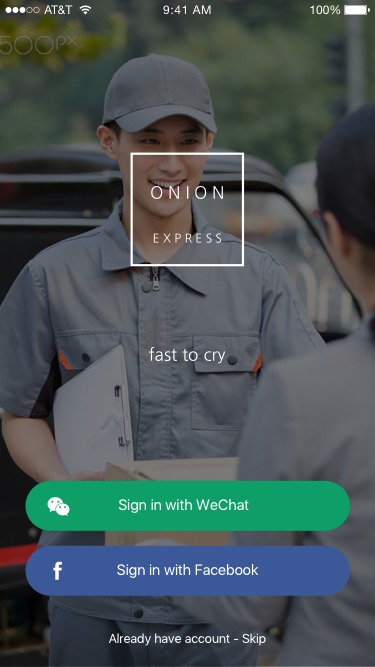
\includegraphics[width=3in]{DocumentRes/Login.png}
  \caption{Log in}
\end{figure}
This is the login page of our app, for convenience, users can log in via WeChat or
Facebook, which is the popular socail account around the world. Through the
account, we will record user's infomation in the server, and can sync data to
provide a better user experience.

\subsection{Main Page}
\begin{figure}[htbp]
  \centering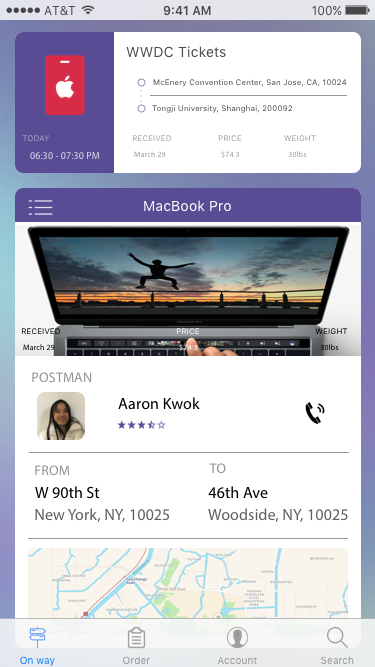
\includegraphics[width=3in]{DocumentRes/OnWay.png}
  \caption{On way}
\end{figure}
This is the main page of our app. It shows the user at all glance all the
current package, and click on the user after the show the details of the
package. Details of the courier to provide a contact, historical evaluation,
and the location of real-time display on the map, easy to track users.
In addition, the basic information about the package is provided:
including estimated time of arrival, delivery costs and weight.

\subsection{Search Page}
\begin{figure}[htbp]
  \centering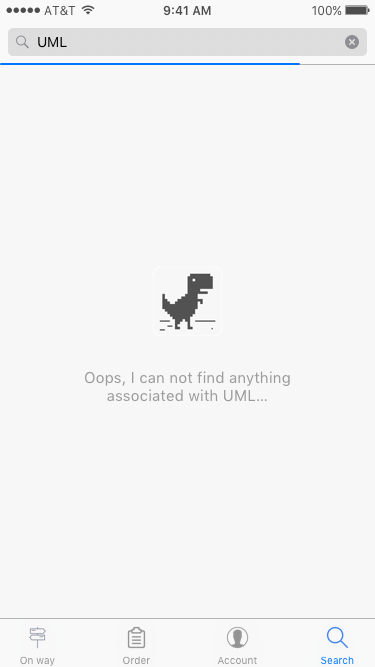
\includegraphics[width=3in]{DocumentRes/Search.png}
  \caption{Search}
\end{figure}
This is the search page of our app. User can type everything he/she want to.
And we will search both locally and in the server.

\subsection{Order Page}
\begin{figure}[H]
  \centering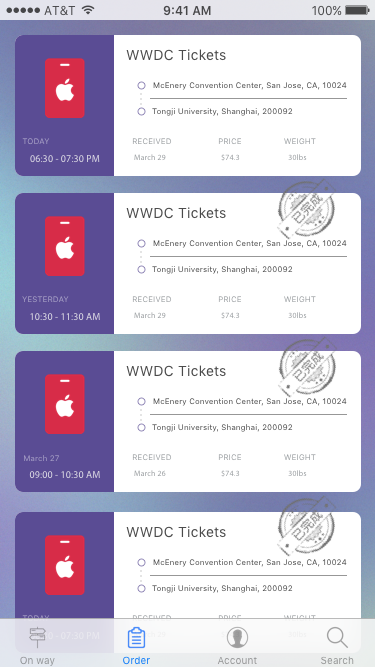
\includegraphics[width=3in]{DocumentRes/Order.png}
  \caption{Order}
\end{figure}
This is the order page of our app. It shows all the packages both on the way and
delivered. Like the main page, it can show details and ordered with timeline.

\subsection{Account Page}
\begin{figure}[H]
  \centering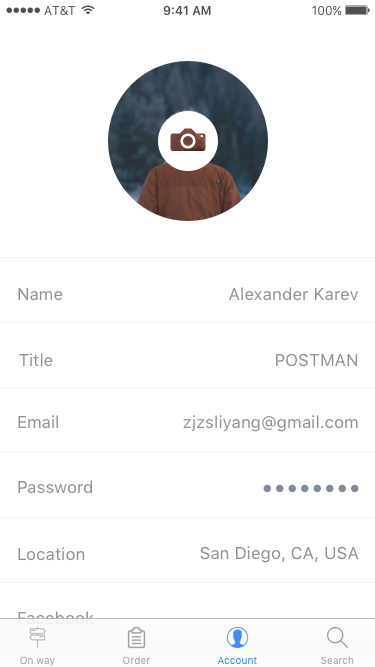
\includegraphics[width=3in]{DocumentRes/Account.png}
  \caption{Account}
\end{figure}
This is the account page of our app. It shoes the basic infomation of users,
including name, title, email, password, location and social account. Users can
change settings there and it's simple and concise。

\section{Website}
There is basic information of the system showed on the page. The services can
be ordered on this website after the user logs in. The custom can search for
their packages' particulars after logging in. In addition, the significant
notations of the Onion Express\textregistered\ are showed on the web page, such us the forbidden
objects etc. Any common browsers of the website can contact the Onion
Express\textregistered\ company and know about the company freely.
\begin{figure}[htbp]
  \centering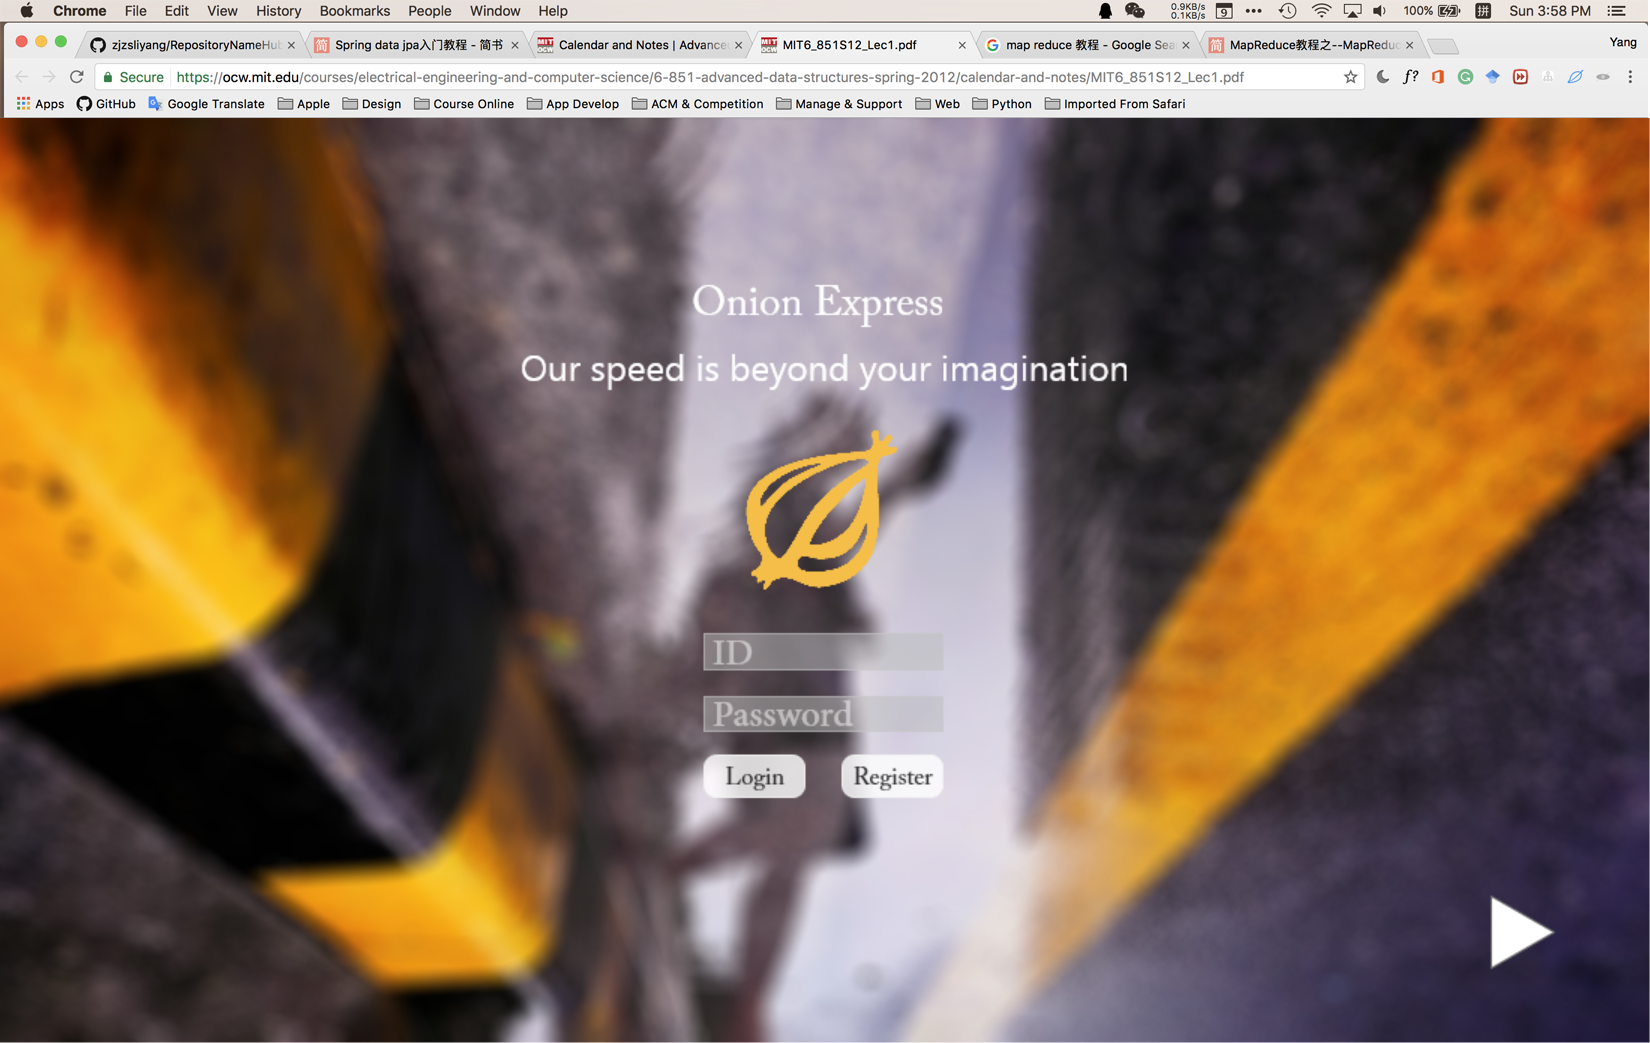
\includegraphics[width=4in]{DocumentRes/index1.png}
  \caption{Index1}
\end{figure}
\begin{figure}[htbp]
  \centering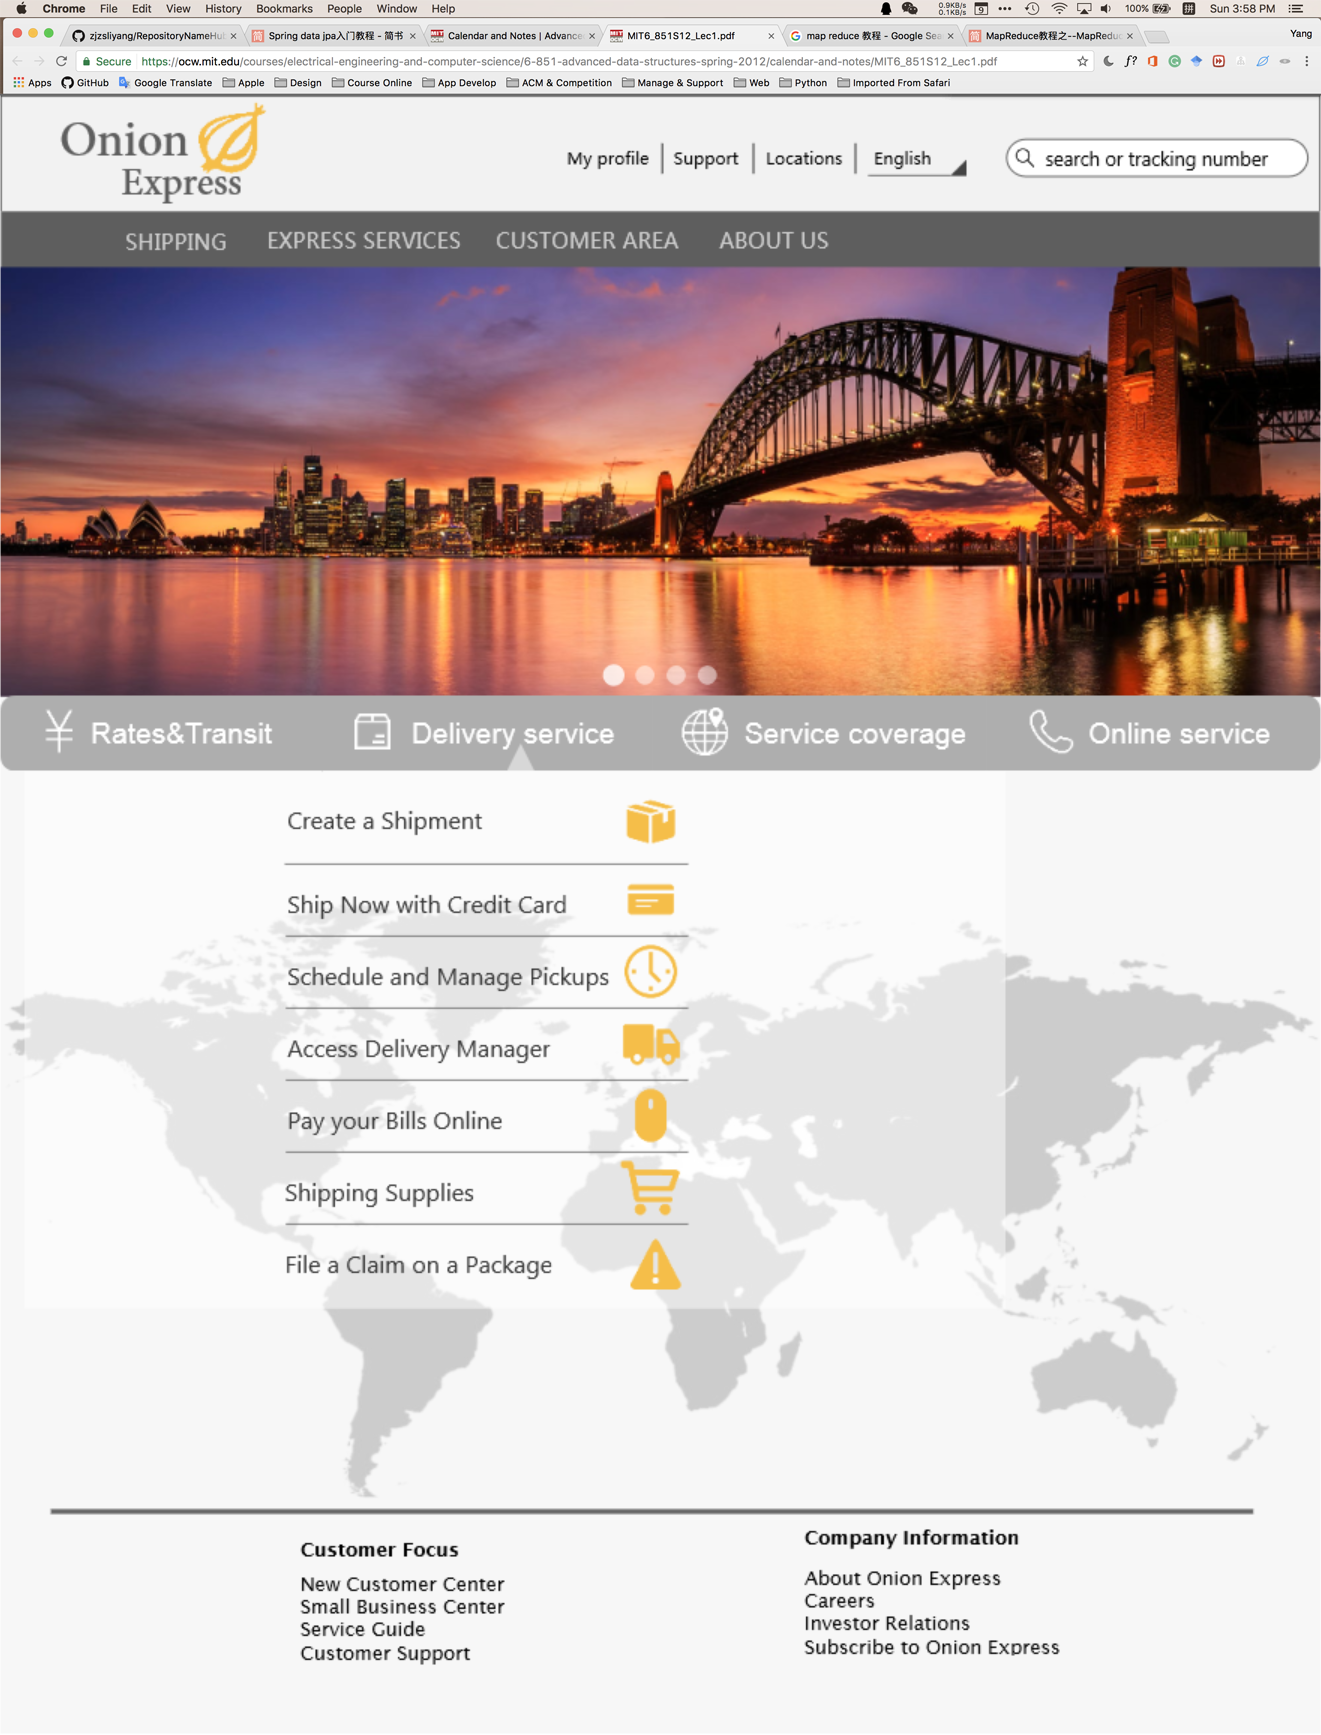
\includegraphics[width=4in]{DocumentRes/index2.png}
  \caption{Index2}
\end{figure}
\begin{figure}[htbp]
  \centering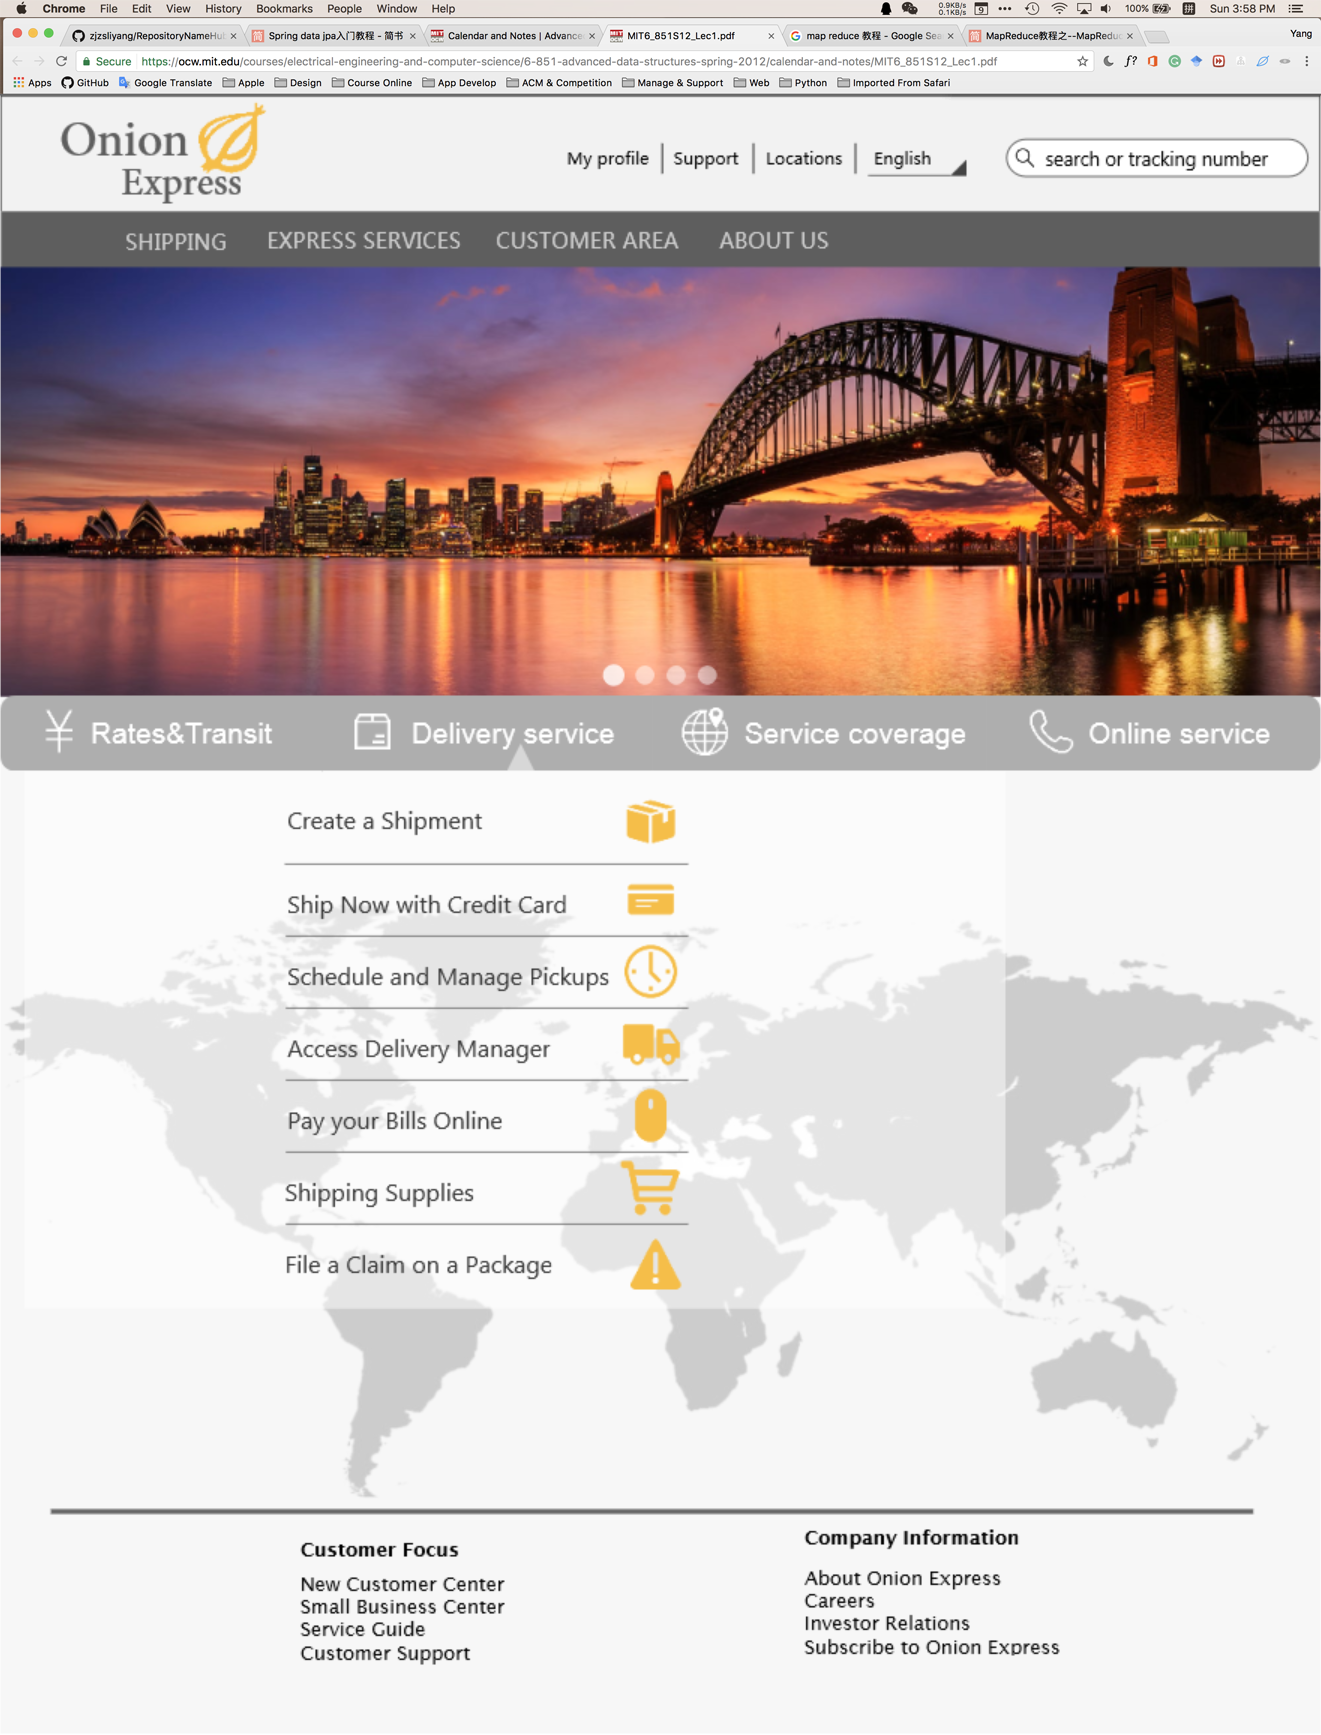
\includegraphics[width=5in]{DocumentRes/index3.png}
  \caption{Index3}
\end{figure}

\chapter{Contributions}
More information, please visit more on \href{https://github.com/zjzsliyang/42003201ObjectOrientedAnalysisAndDesign}{GitHub}
\vspace{3mm}\\
\href{https://github.com/zjzsliyang}{{\color{blue}1452559 Yang LI}} \hspace{17mm} iOS UI, Document\hfill 17\%\\
\href{https://github.com/tjluozhongjin}{{\color{blue}1453645 Zhongjin LUO}} \hspace{5mm} Use Case Diagram, Activity Diagram\hfill 17\%\\
\href{https://github.com/Yghifi}{{\color{blue}1451229 Guohui YANG}} \hspace{4.5mm} Use Case Diagram, Activity Diagram\hfill 17\%\\
\href{https://github.com/Charon0622}{{\color{blue}1552651 Yirui WANG}} \hspace{7mm} Use Case Diagram, Activity Diagram\hfill 17\%\\
{{\color{blue}1552677 Xinying WU} \hspace{8mm} Web UI\hfill 17\%\\
\href{https://github.com/lyqun}{{\color{blue}1552705 Yiqun LIN}} \hspace{11mm} Use Case Diagram, Activity Diagram\hfill 17\%

\begin{thebibliography}{99}
\bibitem{1998}
  830-1998,
  \emph{IEEE Recommended Practice for Software Requirements Specifications},
  IEEE,
  Oct 1998.
\bibitem{2011}
  29148-2011,
  \emph{Systems and software engineering -- Life cycle processes --Requirements engineering},
  ISO/IEC/IEEE International Standard,
  Dec 2011.
\bibitem{Miles}
  Russ Miles, Kim Hamilton,
  \emph{Learning UML 2.0},
  O'REILLY,
  1st edtion,
  April 2006.
\bibitem{Arlow}
  Jim Arlow,
  \emph{UML 2.0 and the Unified Process: Practical Object-oriented Analysis and Design},
  ADDISON WESLEY,
  2nd edition,
  2005.
\bibitem{Wiegers}
  Karl Eugene Wiegers, Joy Beatty,
  \emph{Software Requirements},
  Microsoft Press,
  3rd edition,
  2013.
\bibitem{Larman}
  Craig Larman,
  \emph{Applying UML and Patterns},
  Pearson Education International,
  3rd edition,
  2005.
\bibitem{Bennett}
  Simon J. Bennett, Steve McRobb, Ray Farmer,
  \emph{Object-oriented Systems Analysis and Design Using UML},
  McGraw-Hill Education,
  2nd edition,
  Dec 2001.
\bibitem{TAN}
  Yunjie TAN,
  \emph{Thinking in UML},
  China Water Conservancy Hydropower,
  2nd edition,
  March 2012.
\end{thebibliography}

\end{document}
